\chapter{面向肺鳞癌疗效评估的数字病理分析方法研究}

\section{引言}
新辅助免疫联合化疗已经成为可切除非小细胞肺癌的重要治疗方式，但术后病理评估仍面临两类相互关联的困难。NADIM、CheckMate-816、KEYNOTE-671、AEGEAN 和 CheckMate 77T 等临床研究从新辅助或围术期治疗角度一致支持免疫检查点抑制剂联合化疗在可切除非小细胞肺癌中的应用价值\cite{provencio2020nadim,forde2022checkmate816,wakelee2023keynote671,heymach2023aegean,cascone2024checkmate77t}；然而，治疗反应评估和风险分层仍面临挑战，尤其是未达到病理完全缓解的患者。CheckMate-816的长期随访结果显示，non-pCR患者约占全部接受治疗者的75\%，其5年总生存率仅为55.7\%，而pCR患者为95.3\%，凸显了这一主要人群的高风险属性。当前以 RVT 为代表的病理评估框架虽能提供重要预后信息。MPR 作为新辅助治疗后的替代终点已被系统提出，IASLC 也进一步规范了切除标本的病理评估口径\cite{hellmann2014mpr,travis2020iaslc}。
RVT 能够反映肿瘤退缩程度，却不能完整表征新辅助免疫化疗后形成的肿瘤--免疫生态。尤其是肿瘤边界附近的中性粒细胞聚集与较大空间范围内的淋巴细胞浸润，可能分别代表局部免疫抑制和持续抗肿瘤免疫，但这些空间表型在常规病理实践中难以稳定量化。以RVT为代表的病理评估框架在临床使用时主要面临以下两个主要问题：
第一，残余活性肿瘤（residual viable tumor, RVT）需要病理医师在多张全切片图像（whole-slide image, WSI）上综合估计活性肿瘤、坏死和治疗后间质的比例，耗时较长且容易受到观察者经验和区域异质性的影响。第二，病理完全缓解（pathological complete response, pCR）和主要病理缓解（major pathological response, MPR）均以离散阈值概括连续的治疗反应谱，难以进一步区分具有残余肿瘤患者的术后风险。

此外，仅关注肿瘤消退的基于 RVT 的指标并不能完全捕捉新辅助免疫化疗引起的复杂的免疫-肿瘤相互作用。肿瘤微环境（TME）特征提供了额外的预后信息。免疫浸润的丰度或模式，包括中性粒细胞、淋巴细胞和基质反应，与肺癌的治疗敏感性和生存相关\cite{wu2024coldhot,teijeira2021il8,miao2024neutrophilsnsclc,hu2025neutrophilpd1}。先前的研究表明，富含淋巴细胞的“热”肿瘤与改善的免疫治疗反应相关\cite{wu2024coldhot}，而肿瘤相关的中性粒细胞则导致免疫逃避和不良预后\cite{teijeira2021il8,miao2024neutrophilsnsclc,hu2025neutrophilpd1}。然而，由于其劳动密集型性质和有限的重复性，这些微环境特征在病理实践中并未被常规量化，并且它们在新辅助免疫化疗环境中的预后相关性，特别是在肺鳞状细胞癌（LUSC）中，仍未得到充分定义。
基于人工智能 (AI) 的数字病理学的最新进展使得能够对全切片图像 (WSI) 中的 RVT 和 TME 特征进行可重复、高通量的量化。大规模弱监督 WSI 学习和数据高效多实例学习已经证明，切片级标签可以支持临床级病理分类与跨队列验证\cite{campanella2019clinical,lu2021clam,ilse2018attentionmil,li2021dsmil,shao2021transmil}；层级自监督学习与全切片基础模型进一步表明，联合建模局部细胞形态和全局组织上下文能够提高 WSI 表征的迁移性\cite{chen2022hipt,xu2024gigapath}；在非小细胞肺癌中，深度学习还可从常规 H\&E 图像预测组织学类型与部分分子改变\cite{coudray2018lung}。AI 衍生的 RVT 已证明与仅接受新辅助免疫治疗的患者的病理学家评估和预后价值高度一致\cite{dacic2024lcmc3}。然而，目前尚不清楚人工智能衍生的指标在新辅助免疫化疗（现在是主要的新辅助策略）的背景下是否保留预测效用，以及这些定量特征如何与淋巴结状态等关键临床变量相互作用。与此同时，越来越多的证据表明，TME 内肿瘤和基质免疫细胞的空间组成和组织可以使用基于深度学习的病理模型进行定量表征，并作为肺腺癌的独立预后因素\cite{wang2020compstaining,wang2019convpath}。值得注意的是，基于人工智能的全玻片分析仪能够识别癌症区域、间质和关键 TME 成分，包括肿瘤浸润淋巴细胞、成纤维细胞和内皮细胞，能够描绘 TKI 耐药后 EGFR 突变 NSCLC 的动态微环境变化，并预测随后对基于免疫疗法的治疗的反应\cite{bang2025egfrspatial}。这些发现强调了人工智能衍生的空间 TME 特征在告知免疫治疗反应方面具有更广泛的相关性，并促使它们整合到基于 RVT 的生存模型中，特别是对于非 pCR 人群。
因此，利用国家癌症中心的两个队列（NCC\_Cohort1 和 NCC\_Cohort2）的数据集以及山西省肿瘤医院（SXCH）和深圳肿瘤医院（SZCH）的其他外部队列的数据集，我们开发了一个多尺度 AI 驱动的病理学框架，该框架可以同时量化接受新辅助免疫化疗治疗的 LUSC WSI 中的 RVT 与瘤周免疫细胞密度。这种综合方法旨在加强术后风险分层，特别是非 pCR 患者，并为辅助治疗决策和临床监测提供更有生物学依据的基础。


本章以接受新辅助免疫化疗的肺鳞状细胞癌（lung squamous cell carcinoma, LUSC）患者为研究对象，建立一套模拟病理医师多尺度阅片过程的数字病理框架。该框架首先在 WSI 上识别肿瘤床、活性肿瘤、坏死和正常组织，计算连续的 AI-RVT；随后利用视觉语言基础模型完成多类细胞检测，并按细胞到肿瘤边界的距离构建空间免疫表型；最后分别评价 AI-RVT、单一空间细胞特征及联合免疫表型与无病生存（disease-free survival, DFS）和总生存（overall survival, OS）的关系。与直接输出生存风险的黑箱模型不同，本研究保留区域、细胞类别、空间距离和临床终点之间的对应关系，使每一级结果均可由病理医师追溯核验。

\section{肺鳞癌数字病理分析方法}
\subsection{研究目标与总体技术路线}
本章目标是把肺鳞癌新辅助治疗后病理评价转化为一条可复现的计算链：首先在 WSI 上识别肿瘤床、活性肿瘤、坏死与正常组织并计算连续 AI-RVT；随后利用渐进式视觉语言学习检测肿瘤及免疫--间质细胞；最后以肿瘤边界为参照构建距离分层的空间细胞密度，并分析这些图像指标与病理缓解及患者预后的关系。与单纯追求检测精度不同，该技术路线要求图像层输出能够稳定聚合到切片级和患者级，并能进入临床统计模型。

\subsection{多尺度区域分析与残余肿瘤量化}
病理医师通常先在器官和组织尺度定位病变，再在细胞尺度确认活性肿瘤。若感受野不足，模型难以像医师一样综合更大范围内的组织结构与细胞分布信息，从而对局部区域的细胞类型与病理状态作出可靠判断。为模拟这种“放大--缩小”的阅片过程，本研究以最小尺度图块为中心逐级扩展感受野，生成空间对齐的大尺度训练样本。不同尺度分别建立区域分类分支，并通过空间对齐保持中心位置一致，使尺度变化只改变上下文范围而不改变预测对象。推理时再融合各尺度证据，从而避免单一局部纹理主导区域判断。
推理时，各尺度模型独立输出四类区域得分，再依据对应尺度中病理区域的面积进行加权融合。设第 $s$ 张切片中活性肿瘤、治疗后间质性肿瘤床和坏死区域面积分别为 $A^{(s)}_{\mathrm{tumor}}$、$A^{(s)}_{\mathrm{bed}}$ 和 $A^{(s)}_{\mathrm{necrosis}}$，则切片级 RVT 表示为
\begin{equation}
R_s=\frac{A^{(s)}_{\mathrm{tumor}}}
{A^{(s)}_{\mathrm{tumor}}+A^{(s)}_{\mathrm{bed}}+A^{(s)}_{\mathrm{necrosis}}+\epsilon}.
\end{equation}
设患者共有 $S$ 张可用切片，其患者级 AI-RVT 为
\begin{equation}
R_{\mathrm{patient}}=\frac{1}{S}\sum_{s=1}^{S}R_s.
\end{equation}
这一连续值既可按 10\% 阈值转换为 MPR 标签，也可直接进入 Cox 模型。

\subsection{渐进式视觉语言细胞检测}
目标队列中的细胞精细标注数量有限，且不同公共病理数据集的标签空间并不一致。为避免直接在少量目标域样本上训练导致过拟合，本研究将模型适配拆分为三个连续过程，并严格区分公开病理数据预训练、目标域粗粒度适配和目标域细粒度精调。其核心思想是先学习跨数据集稳定的细胞形态与视觉语言对应关系，再逐步注入目标队列的染色风格、组织结构和细胞类别信息。

\subsubsection{公开医学病理数据预训练}
第一阶段使用 MoNuSAC、CCRCC 和 CoNSeP 等公开医学病理数据集进行多类细胞预训练。其中，MoNuSAC 与同类多器官核数据集为跨组织细胞核分割和分类提供了标准化训练基础\cite{verma2021monusac,gamper2019pannuke,graham2021lizard}。与直接把所有数据的类别编号拼接在一起不同，本研究首先将不同数据集中的类别名称统一映射到细胞语义空间，并将类别名称作为文本提示输入 GLIP 的语言分支。图像编码器负责提取细胞的形态、纹理和局部组织背景，语言编码器则提供可迁移的类别语义；检测头通过区域--文本匹配学习细胞区域与类别短语之间的对应关系。这样做的目的不是让模型记忆某一个数据集的染色或类别编号，而是使其在不同标注体系之间学习较稳定的细胞外观表示，为后续目标域适配提供病理视觉先验。

在实现上，过程一以 GLIP-L 的预训练参数作为基础初始化，并采用与后续目标域训练一致的检测框架和文本提示形式。公开数据预训练阶段主要承担两个作用：一是将自然图像中的开放词汇检测能力迁移到细胞和细胞核等医学目标；二是利用多个公开数据集的形态变化增加训练样本的覆盖范围，减弱模型对单一数据集染色风格和标注习惯的依赖。由于该阶段使用的是公开医学数据而非本研究队列的测试图块，因此不会直接泄漏目标测试图像的实例标注。

\subsubsection{目标域粗粒度适配}
第二阶段在 NCC\_Cohort1 的目标域 WSI 上继续训练。我们从 7 例患者的 WSI 中提取 1,318 个图块，使用 Tumor 和 Stromal 两类相对可靠的粗粒度区域标签进行域内适配。此时不急于加入所有细粒度细胞类别，而是先让图像编码器和检测头适应本研究队列的 H\&E 染色、组织背景、肿瘤--间质结构及图块尺度。这样可以避免在细粒度标注尚不充分时，把类别遗漏或边界不确定性过早传播到整个模型。

\subsubsection{目标域细粒度精调}
第三阶段从完整标注区域以重叠采样方式获得 938 个 $224\times224$ 图块，对 Tumor cell、Lymphocyte、Neutrophil、Eosinophil、Plasma Cell、Endothelial Cell、Fibroblast 和 Histiocyte 八类细胞进行精调；小于图块尺寸的区域采用黑色填充。另从测试数据中按相同策略选取 8 个图块用于检测性能评价。细粒度精调阶段使用高质量逐实例标注，重点优化类别判别、实例边界和密集细胞场景中的区域匹配关系。

\subsection{肿瘤周围细胞提取与空间密度}
对存在残余肿瘤的 WSI，选取面积最大的肿瘤区域作为代表灶，并沿其轮廓提取周边图块；未检测到活性肿瘤时，则以最大间质区域为中心提取半径为 5 个图块的邻域。细胞检测结果除类别和置信度外，还记录细胞相对最近肿瘤边界点的水平、垂直偏移 $(V_x,V_y)$，仅保留置信度不低于 0.5 的检测目标。细胞到边界的欧氏距离为
\begin{equation}
d=\sqrt{V_x^2+V_y^2}.
\end{equation}
由于 $V_x$ 和 $V_y$ 均限制在 $500\,\mu\mathrm{m}$ 内，可测最大距离约为 $707\,\mu\mathrm{m}$。因此，本研究以 $50\,\mu\mathrm{m}$ 为步长，在 $50$--$700\,\mu\mathrm{m}$ 范围内建立累积径向区域。若肿瘤边界周长为 $P$，向外扩张距离为 $d$，则依据 Minkowski--Steiner 展开公式估计周边面积
\begin{equation}
A(d)=P\,d+\pi d^2,
\end{equation}
相应细胞密度为
\begin{equation}
\rho_c(d)=\frac{N_c(d)}{A(d)},
\end{equation}
其中 $N_c(d)$ 为类别 $c$ 在距离 $d$ 内的检测数。患者级密度由其全部切片对应密度取平均得到。嗜酸性粒细胞在研究队列中的检出频率过低，因此不进入后续生存分析；空间预后分析仅纳入 AI-RVT 大于 0 的残余肿瘤患者。

\subsection{端到端病理分析流程}
以上所述的图块生成与染色归一化、多尺度分类与面积加权融合流程可以整合绘制为一个整体流程图，即图~\ref{fig:lung_pipeline}。以“病理阅片逻辑”为主线，自左向右依次呈现多尺度阅片示意、WSI 图块化与尺度对齐、各尺度分类器训练与推理，以及基于面积占比的加权融合与 AI-RVT 计算。该流程将 WSI 的关键处理步骤进行智能化、自动化串联，可在减少人工逐张阅片负担的同时稳定输出可用于统计分析的量化结果。

\begin{figure}[tb]
  \centering
  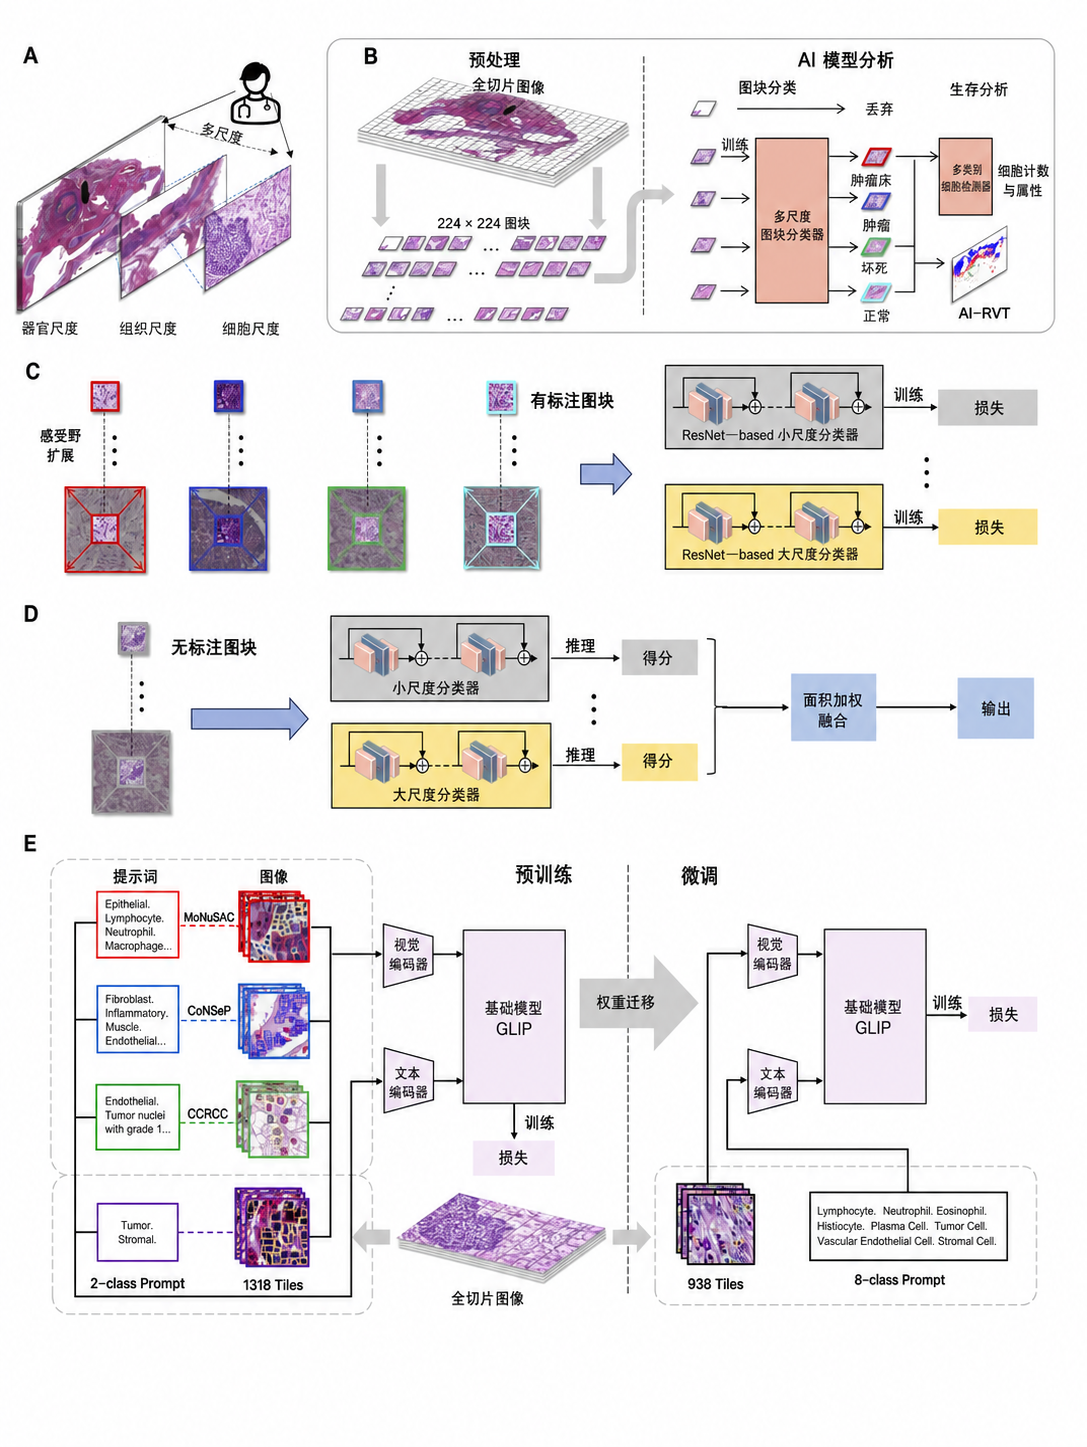
\includegraphics[width=0.88\textwidth,height=0.58\textheight,keepaspectratio]{figures/lung_image8_zh.png}
  \caption{多尺度 WSI 分析与细胞检测流程}
  \label{fig:lung_pipeline}
\end{figure}
图~\ref{fig:lung_pipeline} 将本章的两条技术路径置于同一分析框架中。（A--D）对应区域级分析：首先模拟病理医师由低倍到高倍的阅片过程，再把超大尺寸 WSI 切分为空间对齐的多尺度图块；不同尺度分类器分别判断活性肿瘤、肿瘤床、坏死和正常组织，最终依据各类区域的面积占比完成切片级与患者级 AI-RVT 计算。该流程强调局部细胞形态必须结合较大范围的组织结构进行解释，因而能够减少单尺度图块在肿瘤--间质交界处产生的类别混淆。\par 图中（E）对应细胞级分析。GLIP 检测器依次经历公共多类细胞核数据预训练、目标域肿瘤/间质粗粒度适配以及八类细胞精细标注训练，使通用视觉语言表征逐步适应肺鳞癌 H\&E 图像。两条路径在输出层面形成互补：区域分支给出残余肿瘤负荷，细胞分支提供肿瘤周围免疫和间质细胞的类别与坐标，二者共同构成后续生存分析所需的可解释变量。数据集名称、类别提示词和模型名称作为实际训练输入保留英文。

\section{实验设置}
本节只说明数据来源、标注与预处理、模型训练参数以及临床统计口径；算法设计动机和公式已在上一节给出，所有性能数值、对照表和显著性检验结果统一置于“实验结果与分析”，避免设置与结论交叉。

\subsection{数据集准备}
研究数据来自国家癌症中心（National Cancer Center, NCC）、山西省肿瘤医院（Shanxi Cancer Hospital, SXCH）和深圳市肿瘤医院（Shenzhen Cancer Hospital, SZCH），总体设计如图 \ref{fig:lung_study_design} 所示。

训练数据队列 NCC\_Cohort1 包含 20 例患者的 251 张病理医师精细标注 WSI，用于训练多尺度区域分类器和构建域内细胞检测数据。外部验证数据队列 SXCH 包含 28 例患者的 192 张 WSI，用于评价 AI-RVT 与病理医师视觉评估结果 VIS-RVT 在切片级和患者级的一致性。独立测试数据由 NCC\_Cohort2 的 51 例患者和 SZCH 的 32 例患者构成；在预后分析中进一步合并 NCC\_Cohort1 的 20 例患者，最终形成 103 例患者的生存队列。该队列中 78 例为 non-pCR 患者，占 75.7\%，是术后风险分层的重点对象。具有完整患者级 VIS-RVT 和 AI-RVT 的 84 例患者被纳入 MPR 一致性分析。
数据集预处理细节：医生使用openslide工具手动在WSI图片文件上进行标注，由于一般的WSI图都十分庞大，长宽一般为数十万像素到上百万像素尺度，进行大范围内的逐个的实例级标注是不现实的，过于耗费人力和时间。实验医生只进行两种标注任务：1.以整张WSI的缩略图为依据，在整张WSI图内画圈方式圈出多个区域，然后标明每个区域具体的区域类型（比如瘤床区，坏死区，肿瘤区） 2.对采样出的大量小范围的病理切片区域，进行细致的逐实例标注。标注任务2与前一个标注任务相比，更要求细致、精准、无遗漏，而不苛求过大的实例量。前期实验中发现对于标注任务2以及基于它的细胞检测模型训练，只需要每类数百甚至数十个实例就足以取得比较满意的最终检测效果。

\subsection{标注任务与数据预处理}
由于一般的 WSI 图像十分庞大，长宽通常达到数十万像素甚至上百万像素尺度，在整张切片上逐个完成实例级标注并不现实，会消耗大量人力和时间。因此，实验医生通常需要区分两类标注任务。第一类是在整张 WSI 的缩略图上，以闭合曲线或多边形圈出若干区域，并为每个区域指定区域类型，例如肿瘤床区、坏死区或活性肿瘤区。第二类是对采样得到的大量小范围病理图块进行细致的逐实例标注，为每一个可辨认的细胞或细胞核勾画独立轮廓。与区域级标注相比，第二类任务要求更细致、精准并尽量避免遗漏，但不以覆盖尽可能多的实例为目标。前期实验表明，对于逐实例标注及基于这些标注训练的细胞检测模型，每一类只需要数百个甚至数十个质量可靠的实例，通常就能够取得较为稳定的最终检测效果。

两类标注的差异会直接影响检测模型所接收的监督信号。图 \ref{fig:annotation_task_comparison} 给出了同一类病理图块的对照示例，其中裁剪区域内的绿色实例来自 GeoJSON 标注中的“淋巴细胞（Lymphocyte）”类别。A 中这些细胞虽然在图像中客观存在，但没有全部被逐一勾画；B 则对相应细胞补充了独立的实例轮廓。对于采用实例检测或实例分割损失的训练流程，如果未标注区域被直接编码为背景或参与负样本匹配，A 中未被勾画的淋巴细胞就可能被模型当作背景，从而同时产生漏检倾向和前景--背景监督冲突。A 表示监督信息不完整，其中未勾画的淋巴细胞会被错误编码为负样本；B 通过完整实例轮廓提供更明确的“一个细胞对应一个实例”的正向约束。因此，本研究在构建细胞检测训练集时优先使用小图块中的高质量逐实例标注，并将区域级标注主要用于 WSI 组织区域分类和多尺度上下文建模。

\begin{figure}[tb]
  \centering
  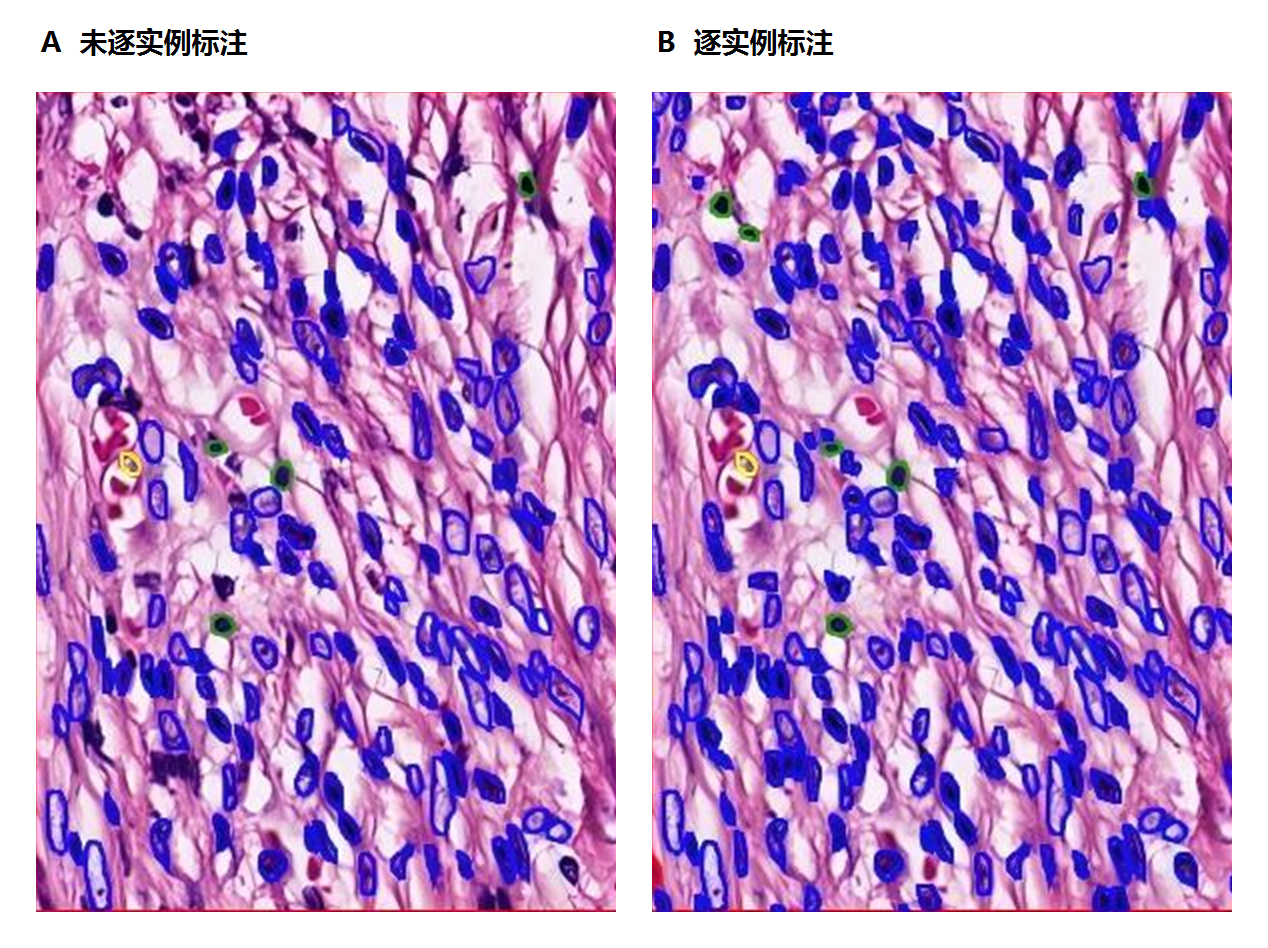
\includegraphics[width=0.76\textwidth]{figures/annotation_task_comparison_recrop_20260824.png}
  \caption{两种实例标注完整性对比}
  \label{fig:annotation_task_comparison}
\end{figure}
图~\ref{fig:annotation_task_comparison} 中，A 表示未完成逐实例标注的版本，B 表示完成逐实例标注的版本；绿色轮廓标出淋巴细胞实例。A 中可见细胞未被全部转化为独立实例轮廓，若训练流程将未标注区域作为背景处理，可能造成前景细胞与背景标签之间的监督冲突；B 为细胞检测模型提供了更完整的实例级正样本。

\subsubsection{WSI 图块生成与染色归一化}
原始 WSI 统一重采样至 20 倍放大倍率，对应约 $0.5\,\mu\mathrm{m}/\mathrm{pixel}$。病理医师以闭合多边形标注肿瘤床、活性肿瘤、坏死和正常区域，程序将 WSI 划分为互不重叠的 $224\times224$ 像素图块。每个图块先转换为灰度图；若亮度范围低于完整动态范围的 35\%，则判定其主要为空白并剔除。对于其余图块，计算四类病理区域的面积占比，仅当某一类别覆盖超过 60\% 时才赋予相应标签，否则舍弃，以减少边界混合图块引入的监督噪声。该流程共获得 975,359 个训练图块。

跨中心染色差异采用 Vahadane 方法进行归一化。该方法借助非负矩阵分解将图像表示为染色浓度矩阵与颜色基矩阵，再把目标切片的颜色基对齐至参考切片并重建图像。与简单颜色直方图匹配相比，这一过程更有利于保留细胞核和间质纹理，同时降低不同中心制片流程造成的颜色偏移。

\subsection{多尺度区域分类配置}
原始 WSI 统一重采样到 20 倍放大倍率（约 $0.5\,\mu\mathrm{m}/\mathrm{pixel}$），以 $224\times224$ 像素为基本图块。病理区域覆盖率超过 60\% 时才赋予类别标签，亮度动态范围不足 35\% 的空白图块予以剔除。多尺度分类器均采用 ResNet-101，优化器为 SGD，基础学习率为 $10^{-4}$，批大小为 4，损失函数为带类别权重的多类别交叉熵。类别权重用于增加稀少活性肿瘤图块在训练中的贡献。为保证尺度消融只反映感受野差异，各尺度使用一致的患者级划分、中心坐标、染色归一化和训练轮次；多尺度结果先在图块级独立输出，再按组织面积完成切片级融合。

\subsection{渐进式细胞检测配置}
细胞检测以 GLIP-L 为视觉语言骨架，保持“公开病理预训练--目标域粗粒度适配--目标域细粒度精调”的三阶段顺序。过程一使用 MoNuSAC、CCRCC 和 CoNSeP 等公开数据，并先统一不同数据集的细胞语义名称；过程二从 NCC\_Cohort1 的 7 例患者中提取 1,318 个图块，以 Tumor/Stromal 粗粒度标签完成染色和组织背景适配；过程三从完整逐实例标注区域重叠采样 938 个 $224\times224$ 图块，训练 Tumor cell、Lymphocyte、Neutrophil、Eosinophil、Plasma Cell、Endothelial Cell、Fibroblast 和 Histiocyte 八类细胞。另按相同预处理策略固定 8 个测试图块用于检测评价。与渐进式模型比较的通用 GLIP 和 Mask R-CNN 对照使用相同目标域训练/测试划分，避免数据量差异成为混杂因素。

\subsection{临床评价指标与统计分析}
本章使用的肺鳞癌数字病理数据与前几章的 patch 级核检测分割数据不同。该工作更接近临床队列研究，并以患者、切片或全切片图像为分析单位，重点评估 AI 量化指标与病理缓解程度、免疫细胞密度、无病生存和总生存之间的关系。因此，该章实验需要同时考虑图像处理流程和临床统计流程。

这类数据的特殊性在于，模型输出构成临床指标计算的中间表征层，并进一步汇总为患者级定量指标。例如，残余可存活肿瘤比例需要由组织区域识别结果推导，肿瘤周围免疫细胞密度需要由细胞检测结果和空间边界关系共同决定。相比检测或分割 benchmark，这类研究更加重视量化指标的可解释性、稳定性和临床相关性。

第五章采用独立的 Lung-AI 图像资源，正文已分别说明研究队列、区域分类、AI-RVT 与 VIS-RVT 一致性、连续 RVT 风险分析以及肿瘤周围免疫细胞联合分层。该实验的可复现性依赖三个关键环节：第一，训练、验证和预后测试患者必须按原研究设计隔离；第二，RVT 需要先在切片级进行面积加权，再聚合到患者级；第三，免疫细胞密度必须记录相对于肿瘤边界的距离范围，确保 $50\,\mu\mathrm{m}$ 和 $700\,\mu\mathrm{m}$ 的统计量具有一致定义。

本章涉及的临床统计指标包括组间差异、相关性分析、ICC 一致性、风险比以及生存曲线等。这些统计分析用于检验 AI 量化指标与病理评估和患者结局之间的稳定关系。对于这类实验，模型性能的最终价值体现在能否形成可解释的临床分层，而不是单纯在图像层面取得高分。

研究以 DFS 和 OS 为临床终点。RVT 同时以两种方式进入分析：一是采用 10\% 阈值区分 MPR 与 non-MPR，二是保留连续比例，以减少阈值二分造成的信息损失。组间生存差异采用 Kaplan--Meier 曲线和 log-rank 检验；DFS 使用标准 Cox 比例风险模型；由于 OS 事件数较少，OS 多变量分析采用 Firth 惩罚 Cox 回归，以降低小样本偏倚并提高风险比估计的稳定性。所有患者级 RVT 均由该患者全部可用切片的 RVT 百分比取算术平均得到。

\section{实验结果与分析}
\subsection{标注完整性实验}
为了定量说明逐实例标注完整性对模型评价的影响，本研究进一步整理同一肺部病理验证任务的两批实验结果。图中 A 表示未完成逐实例补充的标注状态，B 表示经过补充、实例覆盖更完整的标注状态。这里的 A/B 是对标注版本的区分，采用的模型是一致的，都是GLIP-L带有分割头和检测头的标准版本。

表~\ref{tab:annotation_ab_full_metrics} 汇总了两批结果的主要指标。与 A 相比，B 的 Dice、AJI、Diceobj、PQ、F1 和 mAP 均更高。也就是说，在这组实际历史评测中，补充逐实例标注后，模型输出与金标准之间的实例匹配和整体检测统计更加充分；若只观察单一像素级指标，则可能低估标注完整性带来的影响。

\begin{table}[htbp]
  \centering
  \caption{标注完整性对总体性能的影响}
  \label{tab:annotation_ab_full_metrics}
  \resizebox{\textwidth}{!}{%
  \begin{tabular}{llrrrrrrr}
    \toprule
    版本 & 标注含义 & 图块数 & Dice & AJI & Diceobj & PQ & F1 & mAP \\
    \midrule
    A & 未完成逐实例补充 & 8 & 0.709 & 0.433 & 0.710 & 0.328 & 0.668 & 0.2884 \\
    B & 补充完整逐实例标注 & 8 & 0.766 & 0.450 & 0.750 & 0.350 & 0.748 & 0.3750 \\
    \bottomrule
  \end{tabular}}
\end{table}

为了更直观地呈现差异，表~\ref{tab:annotation_ab_delta} 进一步给出了 B 相对于 A 的绝对变化量和相对变化率。B 的 Dice 提高了 0.057，Diceobj 提高了 0.040，AJI 提高了 0.017，PQ 提高了 0.022，F1 提高了 0.080，mAP 提高了 0.0866；其中 mAP 的相对提升达到约 30.0\%，F1 的相对提升约为 12.0\%。这些变化说明，遗漏的细胞实例不仅会减少监督信息，还会改变预测结果与真实实例之间的匹配关系，使评价结果对细胞的检出能力和实例对应关系更加敏感。

\begin{table}[htbp]
  \centering
  \caption{补全实例标注前后的指标变化}
  \label{tab:annotation_ab_delta}
  \begin{tabular}{lrrrr}
    \toprule
    指标 & A & B & 绝对变化（B-A） & 相对变化 \\
    \midrule
    Dice & 0.709 & 0.766 & +0.0570 & +8.0\% \\

    AJI & 0.433 & 0.450 & +0.0170 & +3.9\% \\
    Diceobj & 0.710 & 0.750 & +0.0400 & +5.6\% \\
    PQ & 0.328 & 0.350 & +0.0220 & +6.7\% \\
    F1 & 0.668 & 0.748 & +0.0800 & +12.0\% \\
    mAP & 0.2884 & 0.3750 & +0.0866 & +30.0\% \\
    \bottomrule
  \end{tabular}
\end{table}

上述结果与前文的机制分析相互印证：在 A 中，图像中客观存在但没有被逐一勾画的淋巴细胞可能在训练或评价过程中被当作背景，因而造成前景与背景监督信号混杂；在 B 中，相应淋巴细胞被补充为独立实例，模型输出与金标准之间的实例级对应关系得到更完整的统计。本文将表~\ref{tab:annotation_ab_full_metrics} 和表~\ref{tab:annotation_ab_delta} 作为标注完整性影响的实验证据和支持性分析，不将其夸大为严格控制所有模型权重变量的因果实验。它至少表明：在相同验证数据规模和评价口径下，标注版本的完整程度足以带来明显的性能差异；因此，后续模型训练应优先采用高质量、少遗漏的逐实例标注，并将区域级标注与实例级标注严格区分。

\subsection{区域分类与细胞检测性能}
图~\ref{fig:lung_region_performance}（a）显示，多尺度模型在肿瘤床、活性肿瘤、坏死和正常组织四类区域上均优于单尺度模型。六次独立实验中，平均 F1 从 $0.532\pm0.005$ 提升至 $0.784\pm0.002$，平均精确率从 $0.584\pm0.003$ 提升至 $0.866\pm0.003$，平均召回率从 $0.486\pm0.003$ 提升至 $0.746\pm0.005$；三项指标的相对提升分别为 47.2\%、48.2\% 和 53.3\%。坏死区域的 F1 从 0.426 提高到 0.792，说明大尺度组织上下文对治疗后结构判定尤为重要。

多类细胞检测以相同训练流程下的 Mask R-CNN 和未经额外病理预训练的 GLIP 为对照。渐进式训练模型在七类非肿瘤细胞上的平均 AP50 为 $66.14\pm0.58$，高于 GLIP 对照的 $53.07\pm2.60$ 和 Mask R-CNN 的 $32.26\pm1.40$。其中浆细胞 AP50 达到 $73.57\pm3.18$，相较 GLIP 对照的 $29.33\pm3.10$ 提升明显；这说明公共病理数据预训练和域内粗粒度适配能够缓解小样本细胞类别的过拟合。

\begin{table}[htbp]
  \centering
  \caption{区域分类与细胞检测总体性能}
  \label{tab:lung_model_performance}
  \resizebox{0.98\textwidth}{!}{%
  \begin{tabular}{llll}
    \toprule
    任务 & 方法 & 指标 & 结果（均值$\pm$标准差） \\
    \midrule
    区域分类 & 单尺度 & 平均 F1 / Precision / Recall & $0.532\pm0.005$ / $0.584\pm0.003$ / $0.486\pm0.003$ \\
    区域分类 & 多尺度 & 平均 F1 / Precision / Recall & $0.784\pm0.002$ / $0.866\pm0.003$ / $0.746\pm0.005$ \\
    细胞检测 & Mask R-CNN & 七类平均 AP50 & $32.26\pm1.40$ \\
    细胞检测 & GLIP（无额外预训练） & 七类平均 AP50 & $53.07\pm2.60$ \\
    细胞检测 & 渐进式训练模型 & 七类平均 AP50 & $66.14\pm0.58$ \\
    \bottomrule
  \end{tabular}}
\end{table}

\begin{figure}[tb]
  \centering
  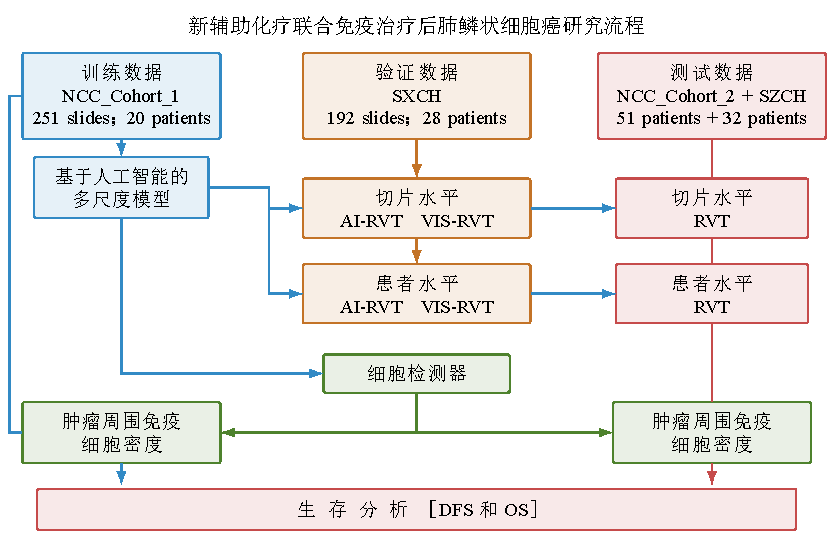
\includegraphics[width=0.92\textwidth]{chapters/lung_study_design_compact.pdf}
  \caption{多中心研究设计}
  \label{fig:lung_study_design}
\end{figure}
图~\ref{fig:lung_study_design} 中，NCC\_Cohort1 用于模型训练，SXCH 用于外部一致性验证，NCC\_Cohort2 与 SZCH 构成独立测试数据；预后分析进一步联合 NCC\_Cohort1。


\begin{table}[htbp]
  \centering
  \caption{多中心队列构成}
  \label{tab:lung_cohorts}
  \resizebox{0.98\textwidth}{!}{%
  \begin{tabular}{llll}
    \toprule
    阶段 & 队列 & 数据规模 & 主要用途 \\
    \midrule
    模型训练 & NCC\_Cohort1 & 20 例，251 张 WSI & 多尺度区域分类与域内细胞建模 \\
    外部验证 & SXCH & 28 例，192 张 WSI & 切片级、患者级 RVT 一致性 \\
    独立测试 & NCC\_Cohort2、SZCH & 51 例、32 例 & 独立测试与空间免疫分析 \\
    预后分析 & NCC\_Cohort1/2、SZCH & 103 例，其中 non-pCR 78 例 & DFS、OS 及联合风险分层 \\
    细胞精调 & NCC\_Cohort1 标注区 & 938 个 $224\times224$ 图块 & 八类细胞检测与分类 \\
    \bottomrule
  \end{tabular}}
\end{table}

\subsection{渐进式训练消融}
\begin{table}[htbp]
  \centering
  \caption{多类细胞检测渐进式训练结果}
  \label{tab:lung_stage_training}
  \resizebox{0.98\textwidth}{!}{%
  \begin{tabular}{p{0.14\textwidth}p{0.26\textwidth}p{0.29\textwidth}p{0.25\textwidth}}
    \toprule
    阶段或对照 & 训练数据与初始化 & 主要作用 & 结果表现 \\
    \midrule
    过程一：公开病理预训练
    & MoNuSAC、CCRCC、CoNSeP；以 GLIP-L 预训练参数初始化
    & 学习跨公开病理数据集的细胞形态、纹理和视觉--语言类别对应关系
    & 为目标域适配提供公开医学视觉先验 \\
    过程二：目标域粗粒度适配
    & NCC\_Cohort1 的 1,318 个图块；Tumor 和 Stromal 两类标签
    & 适应本研究队列的染色、组织背景和肿瘤--间质结构，减少细粒度噪声
    & 为细粒度细胞精调提供目标域初始化 \\
    过程三：目标域细粒度精调
    & 938 个 $224\times224$ 图块；八类细胞逐实例标注
    & 学习细胞类别、实例边界和密集场景下的区域匹配
    & 作为后续定量比较的最佳渐进式训练结果 \\
    无公开医学预训练对照
    & 以通用 GLIP 参数初始化，在目标域训练集上训练，并在验证集上测试
    & 去除公开医学数据预训练，测量通用 GLIP 直接适配病理数据的能力
    & GLIP 对照七类平均 AP50 为 $53.07\pm2.60$ \\
    Mask R-CNN 对照
    & 使用相同目标域数据流程，但不使用视觉--语言预训练
    & 检验性能提升是否来自渐进式视觉语言适配，而非单纯检测头
    & 七类平均 AP50 为 $32.26\pm1.40$ \\
    \bottomrule
  \end{tabular}}
\end{table}


三阶段训练的效果由表~\ref{tab:lung_model_performance} 中的对照结果进一步体现。未经额外公开医学病理数据预训练的 GLIP 在七类非肿瘤细胞上的平均 AP50 为 $53.07\pm2.60$，而采用渐进式公开病理预训练、目标域粗粒度适配和细粒度精调后的模型达到 $66.14\pm0.58$，绝对提高 $13.07$ 个百分点，相对提升约 $24.6\%$。在相同任务下，Mask R-CNN 的七类平均 AP50 为 $32.26\pm1.40$，明显低于两种 GLIP 配置。尤其对于浆细胞等训练样本较少的类别，渐进式训练模型的 AP50 达到 $73.57\pm3.18$，而未额外预训练的 GLIP 对照仅为 $29.33\pm3.10$。这说明公开医学数据预训练首先提供了可迁移的细胞视觉语义，目标域粗粒度适配随后修正染色和组织背景差异，最后的高质量逐实例精调才将这些先验转化为目标队列中的细粒度检测能力。

因此，过程一并不是可有可无的预热步骤，而是整个训练链路中负责建立医学视觉先验的基础环节。若直接从通用 GLIP 权重进入目标域细粒度训练，模型需要在有限的目标域实例上同时学习病理外观、类别语义和实例定位，容易造成小类别过拟合和跨类别混淆。表中的 GLIP 对照与渐进式模型之间的差异，正是对这一训练策略必要性的定量验证。

\subsection{基线临床病理特征}
我们按照中心汇总了 71 例 NCC 患者（NCC\_Cohort1 与 NCC\_Cohort2）、28 例 SXCH 患者和 32 例 SZCH 患者的基线特征，见表 \ref{tab:lung_baseline}。三中心在性别、VIS-RVT、ypT、ypN 和 MPR 分布方面总体可比，年龄分布存在统计学差异（$p=0.031$）。因此，后续生存模型除考察 RVT 和空间免疫指标外，还将治疗后淋巴结状态 ypN 纳入校正。

\begin{table}[htbp]
  \centering
  \caption{患者基线临床病理特征}
  \label{tab:lung_baseline}
  \resizebox{\textwidth}{!}{%
  \begin{tabular}{lcccc}
    \toprule
    特征 & NCC（$N=71$） & SXCH（$N=28$） & SZCH（$N=32$） & $p$ 值 \\
    \midrule
    男性，$n$（\%） & 70（99\%） & 28（100\%） & 29（91\%） & 0.092 \\
    年龄，中位数（Q1，Q3） & 60.00（55.00，65.00） & 63.50（60.50，66.00） & 64.50（59.50，68.50） & 0.031 \\
    VIS-RVT，中位数（Q1，Q3） & 0.03（0.00，0.38） & 0.00（0.00，0.10） & 0.01（0.00，0.13） & 0.300 \\
    \midrule
    ypT 分期 & & & & 0.140 \\
    \quad T0 & 26（37\%） & 13（46\%） & 8（25\%） & \\
    \quad Tis & 1（1.4\%） & 0（0\%） & 0（0\%） & \\
    \quad T1 & 25（35\%） & 11（39\%） & 20（63\%） & \\
    \quad T2 & 13（18\%） & 3（11\%） & 3（9.4\%） & \\
    \quad T3 & 6（8.5\%） & 1（3.6\%） & 0（0\%） & \\
    \quad T4 & 0（0\%） & 0（0\%） & 1（3.1\%） & \\
    \midrule
    ypN 分期 & & & & 0.110 \\
    \quad N0 & 37（52\%） & 23（82\%） & 20（63\%） & \\
    \quad N1 & 19（27\%） & 3（11\%） & 7（22\%） & \\
    \quad N2 & 15（21\%） & 2（7.1\%） & 5（16\%） & \\
    \midrule
    病理缓解 & & & & 0.300 \\
    \quad MPR & 42（59\%） & 21（75\%） & 22（69\%） & \\
    \quad non-MPR & 29（41\%） & 7（25\%） & 10（31\%） & \\
    \bottomrule
  \end{tabular}}
  \vspace{0.3em}

  \raggedright 注：分类变量以 $n$（\%）表示，连续变量以中位数（Q1，Q3）表示；根据变量类型采用 Fisher 精确检验、Kruskal--Wallis 秩和检验或 Pearson 卡方检验。
\end{table}

\subsection{多尺度区域与多类细胞检测结果}
\begin{table}[htbp]
  \centering
  \caption{感受野消融结果}
  \label{tab:lung_receptive_field_ablation}
  \resizebox{\textwidth}{!}{%
  \begin{tabular}{llllll}
    \toprule
    设置 & 感受野/尺度 & 融合策略 & F1（\%）$\uparrow$ & 精确度（\%）$\uparrow$ & 召回率（\%）$\uparrow$ \\
    \midrule
    感受野不足（单尺度/小上下文） & $224\times224$ pixel & 无多尺度融合 & 53.2$\pm$0.5 & 58.4$\pm$0.3 & 48.6$\pm$0.3 \\
    感受野充分（多尺度/大上下文） & $672\times672$ pixel & 多尺度融合 & 78.4$\pm$0.2 & 86.6$\pm$0.3 & 74.6$\pm$0.5 \\
    \bottomrule
  \end{tabular}%
  }
\end{table}



表~\ref{tab:lung_receptive_field_ablation} 比较了单尺度小上下文与多尺度大上下文两种区域分类设置。单尺度模型的平均 F1、精确度和召回率分别为 53.2\% 、58.4\% 和 48.6\%；引入多尺度上下文与融合策略后，三项指标分别提升至 78.4\% 、86.6\% 和 74.6\%。相对于单尺度设置，F1、精确度和召回率的相对提升分别为 47.2\%、48.2\% 和 53.3\%。这表明，单个局部图块提供的组织上下文不足以稳定区分肿瘤床、活性肿瘤、坏死和正常组织，而扩大感受野并进行尺度融合能够利用更完整的组织结构信息，从而同时改善分类的正确性与覆盖能力。

\begin{figure}[tb]
  \centering
  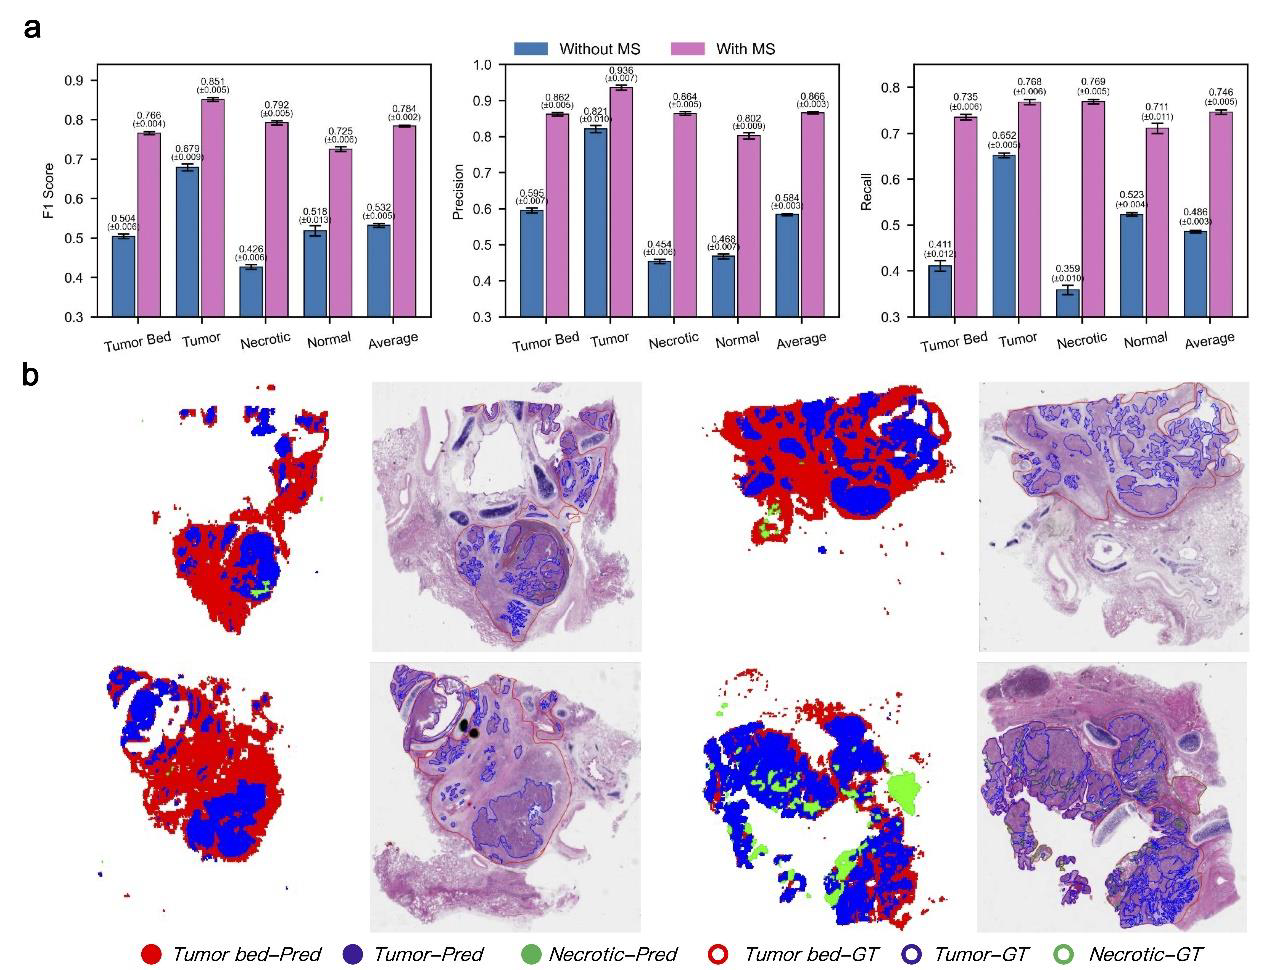
\includegraphics[width=0.76\textwidth]{chapters/lung_fig5_4_ab_20260824.png}
  \caption{多尺度区域分类性能与 WSI 级空间对照}
  \label{fig:lung_region_performance}
\end{figure}
图~\ref{fig:lung_region_performance} 专门考察区域级分析。（a）比较单尺度与多尺度模型在肿瘤床、活性肿瘤、坏死和正常组织四类区域上的 F1、精确率与召回率。引入多尺度上下文后，平均 F1 由 $0.532\pm0.005$ 提升至 $0.784\pm0.002$，平均精确率由 $0.584\pm0.003$ 提升至 $0.866\pm0.003$，平均召回率由 $0.486\pm0.003$ 提升至 $0.746\pm0.005$。其中坏死区域的 F1 从 0.426 提高到 0.792，表明治疗后坏死与间质的区分尤其依赖较大范围组织结构。（b）给出 WSI 级预测与病理标注的空间对照，大面积主体区域总体一致，差异主要集中在活性肿瘤、坏死与治疗后间质交织的边界。该结果说明多尺度模型不仅提高了总体统计量，也使区域面积量化更符合病理阅片中的空间连续性。

\begin{figure}[tb]
  \centering
  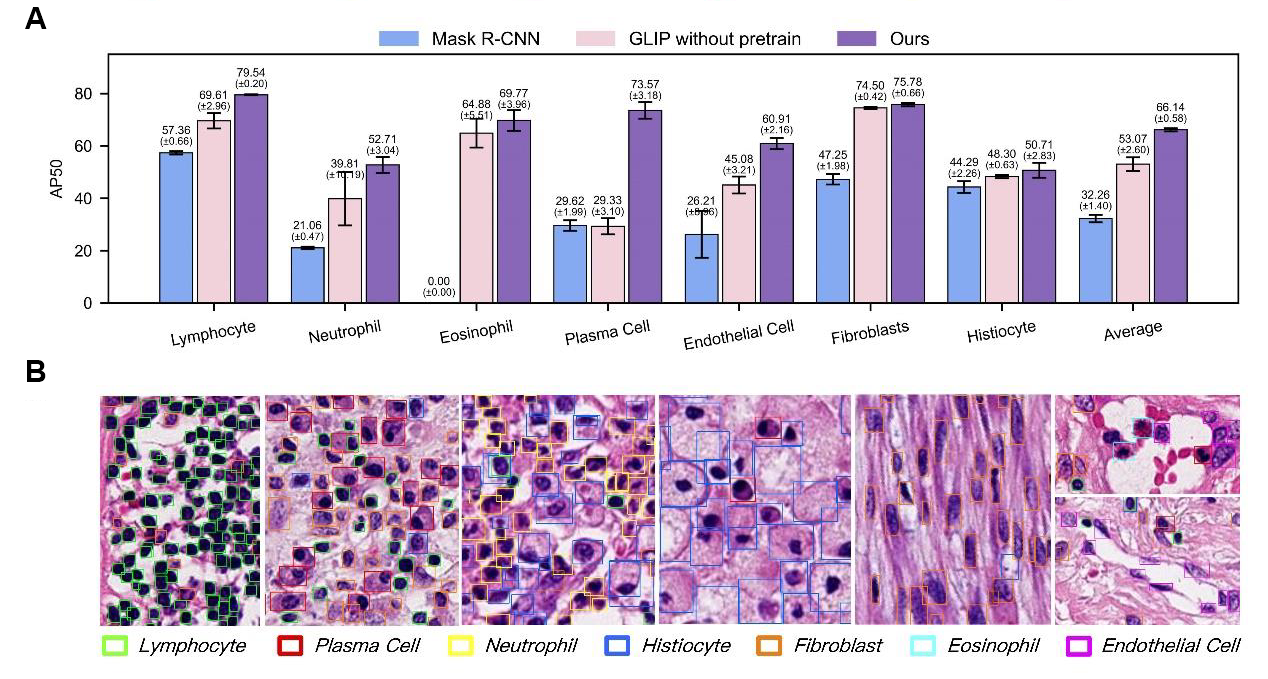
\includegraphics[width=0.84\textwidth]{chapters/lung_fig5_4_cd_precise_ab_20260829.png}
  \caption{多类细胞检测性能与代表性结果}
  \label{fig:lung_cell_performance}
\end{figure}
图~\ref{fig:lung_cell_performance} 转向细胞级分析。（A）比较 Mask R-CNN、未经额外医学预训练的 GLIP 与渐进式训练模型在七类肿瘤周围细胞上的 AP50。渐进式训练模型的七类平均 AP50 为 $66.14\pm0.58$，高于 GLIP 对照的 $53.07\pm2.60$ 和 Mask R-CNN 的 $32.26\pm1.40$；浆细胞等小样本类别的提升尤为明显，验证了公开病理预训练、目标域粗粒度适配和细粒度精调的递进作用。（B）展示多个代表性图块中的分类与定位结果。模型能够在密集、形态相似且染色变化明显的区域同时输出细胞类别和位置，为后续以肿瘤边界为参照的径向密度计算提供实例基础。

\subsection{肺癌细胞联合检测与实例分割结果}
为补充前述细胞检测实验，本研究在原有肺癌数据处理流程上启用原生实例分割头，并固定训练至 4000 次迭代后导出最终模型。评价集包含 8 个 $224\times224$ 病理图块和 669 个逐实例标注。评价标注保留了 9 个历史类别编号，其中嗜酸性粒细胞及其细胞核分别记录为两个标签；因此，本节的目的主要是验证同一视觉语言骨架能否同时输出可用的检测框与非矩形实例掩膜，而不是据此替代患者级临床验证。

表~\ref{tab:lung_native_segmentation_final4000} 给出固定 4000 次迭代模型的最终结果。独立使用 COCO API 复算后，检测任务的 AP、AP50 和 AP75 分别为 0.315、0.604 和 0.278，分割任务的对应指标分别为 0.242、0.514 和 0.175。在置信度阈值固定为 0.5 时，将各类别实例掩膜合并为前景区域后，8 个图块的前景 Dice 宏平均为 0.779，像素汇总 Dice 为 0.773。最终文件共包含 831 个可解码实例掩膜，8 个图块均有检测与分割输出，未发现空掩膜；其中 7 个掩膜的离散轮廓恰好呈矩形，占全部输出的 0.84\%，说明绝大多数输出确实具有实例边界形状，但少量紧凑目标仍可能退化为近似框形轮廓。

\begin{table}[htbp]
  \centering
  \caption{肺癌细胞检测与实例分割的固定终点评价结果}
  \label{tab:lung_native_segmentation_final4000}
  \resizebox{\textwidth}{!}{%
  \begin{tabular}{lcccccccc}
    \toprule
    设置 & BBox AP & BBox AP50 & BBox AP75 & BBox AR100 & Segm AP & Segm AP50 & Segm AP75 & Segm AR100 \\
    \midrule
    历史检测基线 & 0.065 & 0.137 & 0.053 & 0.251 & -- & -- & -- & -- \\
    原生检测--分割模型（4000 次迭代） & 0.315 & 0.604 & 0.278 & 0.461 & 0.242 & 0.514 & 0.175 & 0.327 \\
    \bottomrule
  \end{tabular}}
\end{table}

历史检测基线仅输出边界框，不包含可比较的实例掩膜；其与最终模型之间的训练初始化和监督目标也并非完全相同。因此，表~\ref{tab:lung_native_segmentation_final4000} 中检测指标的差异只能作为流程级描述性对照，不能单独归因于“增加分割头”。可以确认的是，最终联合模型在同一批测试图块上同时给出了有效的检测与分割结果，从而补足了仅依赖框级定位时无法量化细胞轮廓、面积和接触边界的不足。

\begin{figure}[tb]
  \centering
  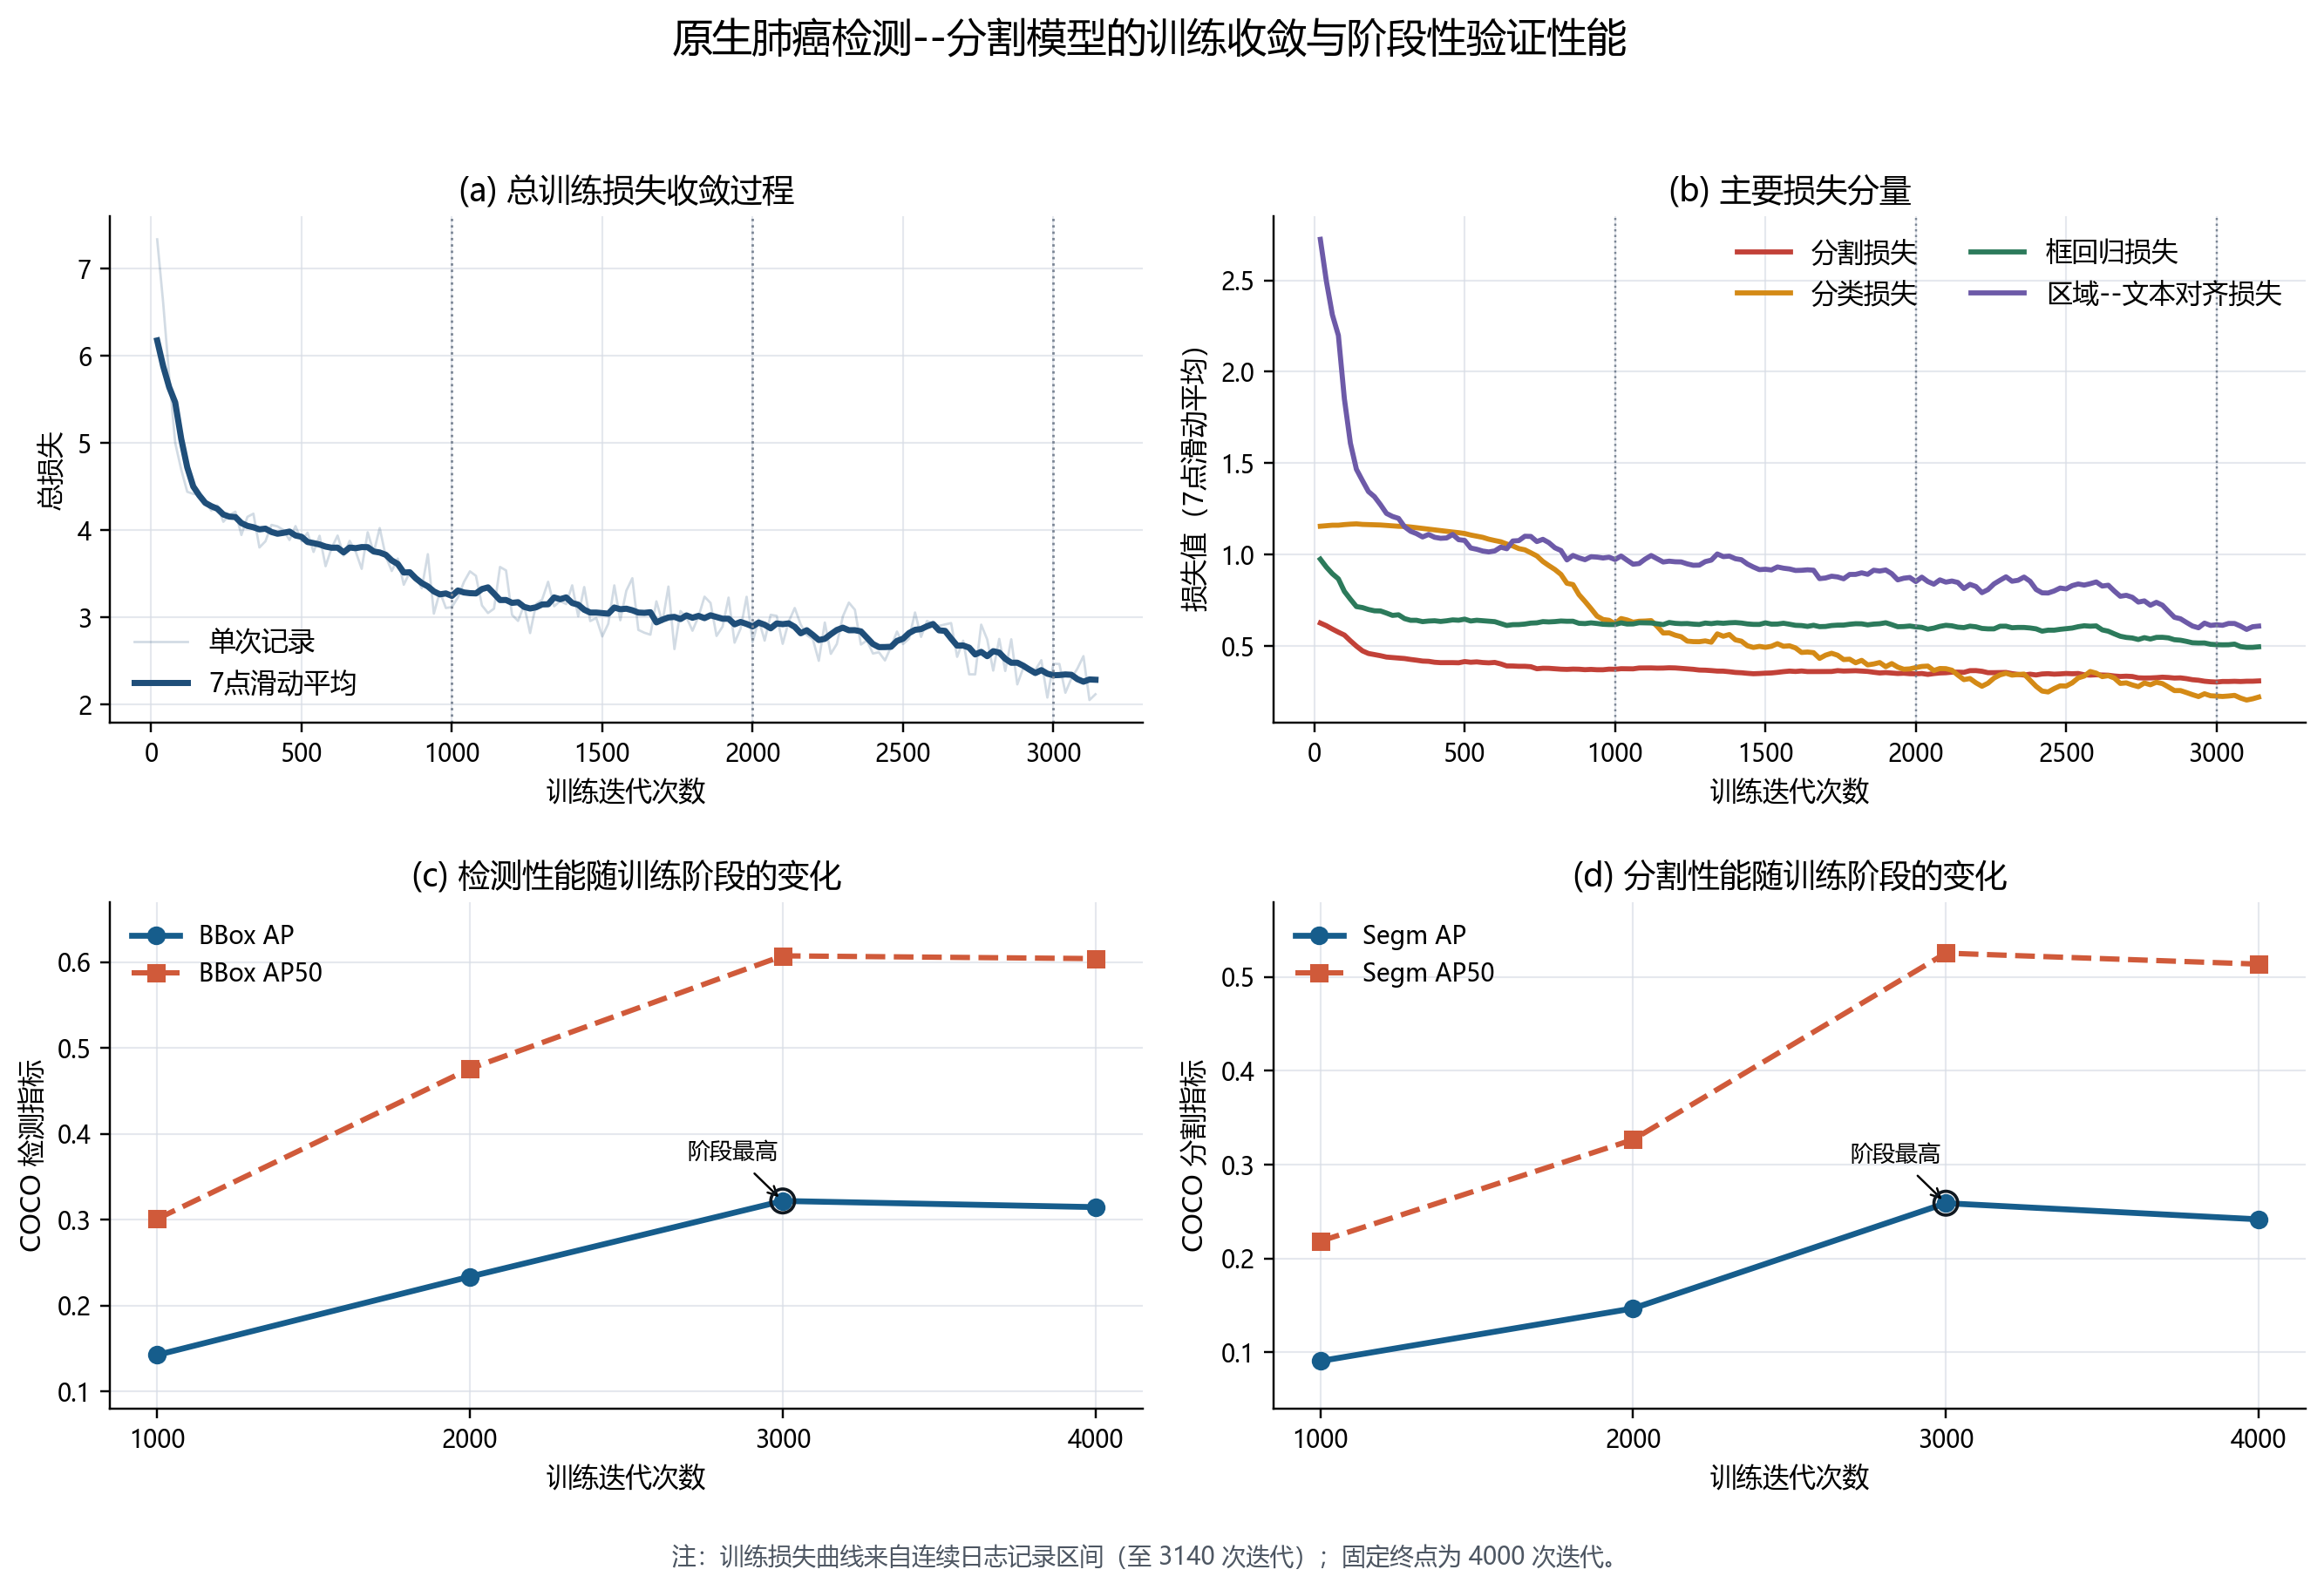
\includegraphics[width=0.96\textwidth]{chapters/lung_native_training_dynamics_20260901.png}
  \caption{原生肺癌检测--分割模型的训练收敛与阶段性性能}
  \label{fig:lung_native_segmentation_curve}
\end{figure}
图~\ref{fig:lung_native_segmentation_curve} 从优化过程和验证性能两个层面展示训练动态。（a）中总损失由训练初期的 6 以上持续下降至 3140 次迭代附近的约 2.3，原始记录虽存在小批量波动，7 点滑动平均曲线仍保持明确的下降趋势。（b）进一步分解主要损失项：区域--文本对齐损失在早期下降最快，分类损失在约 1000 次迭代后继续降低，框回归损失和分割损失则以较平缓的方式收敛。各分量均未出现持续发散或异常突增，说明检测分支、语言对齐分支与实例分割分支能够在联合训练中保持数值稳定。训练损失曲线依据当前保留的连续日志记录至 3140 次迭代，4000 次固定终点则由最终权重的独立评价结果确认。

图~\ref{fig:lung_native_segmentation_curve}（c）和（d）分别给出 1000、2000、3000 和 4000 次迭代时的检测与分割评价结果。检测 AP 从 0.142 提高至 3000 次迭代时的 0.322，分割 AP 同期由 0.091 提高至 0.259；4000 次迭代时两者分别轻微回落至 0.315 和 0.242，AP50 也呈现相同的先升高后轻微下降趋势。由此可见，训练损失继续降低并不必然带来验证集性能同步提高：模型在约 3000 次迭代后已接近小规模目标域数据上的泛化饱和点，继续训练可能强化对训练图块的拟合。为避免依据验证集事后挑选检查点，本文仍以预先规定的 4000 次迭代最终模型作为主结果，而将 3000 次迭代结果仅用于分析训练趋势。


\begin{figure}[tb]
  \centering
  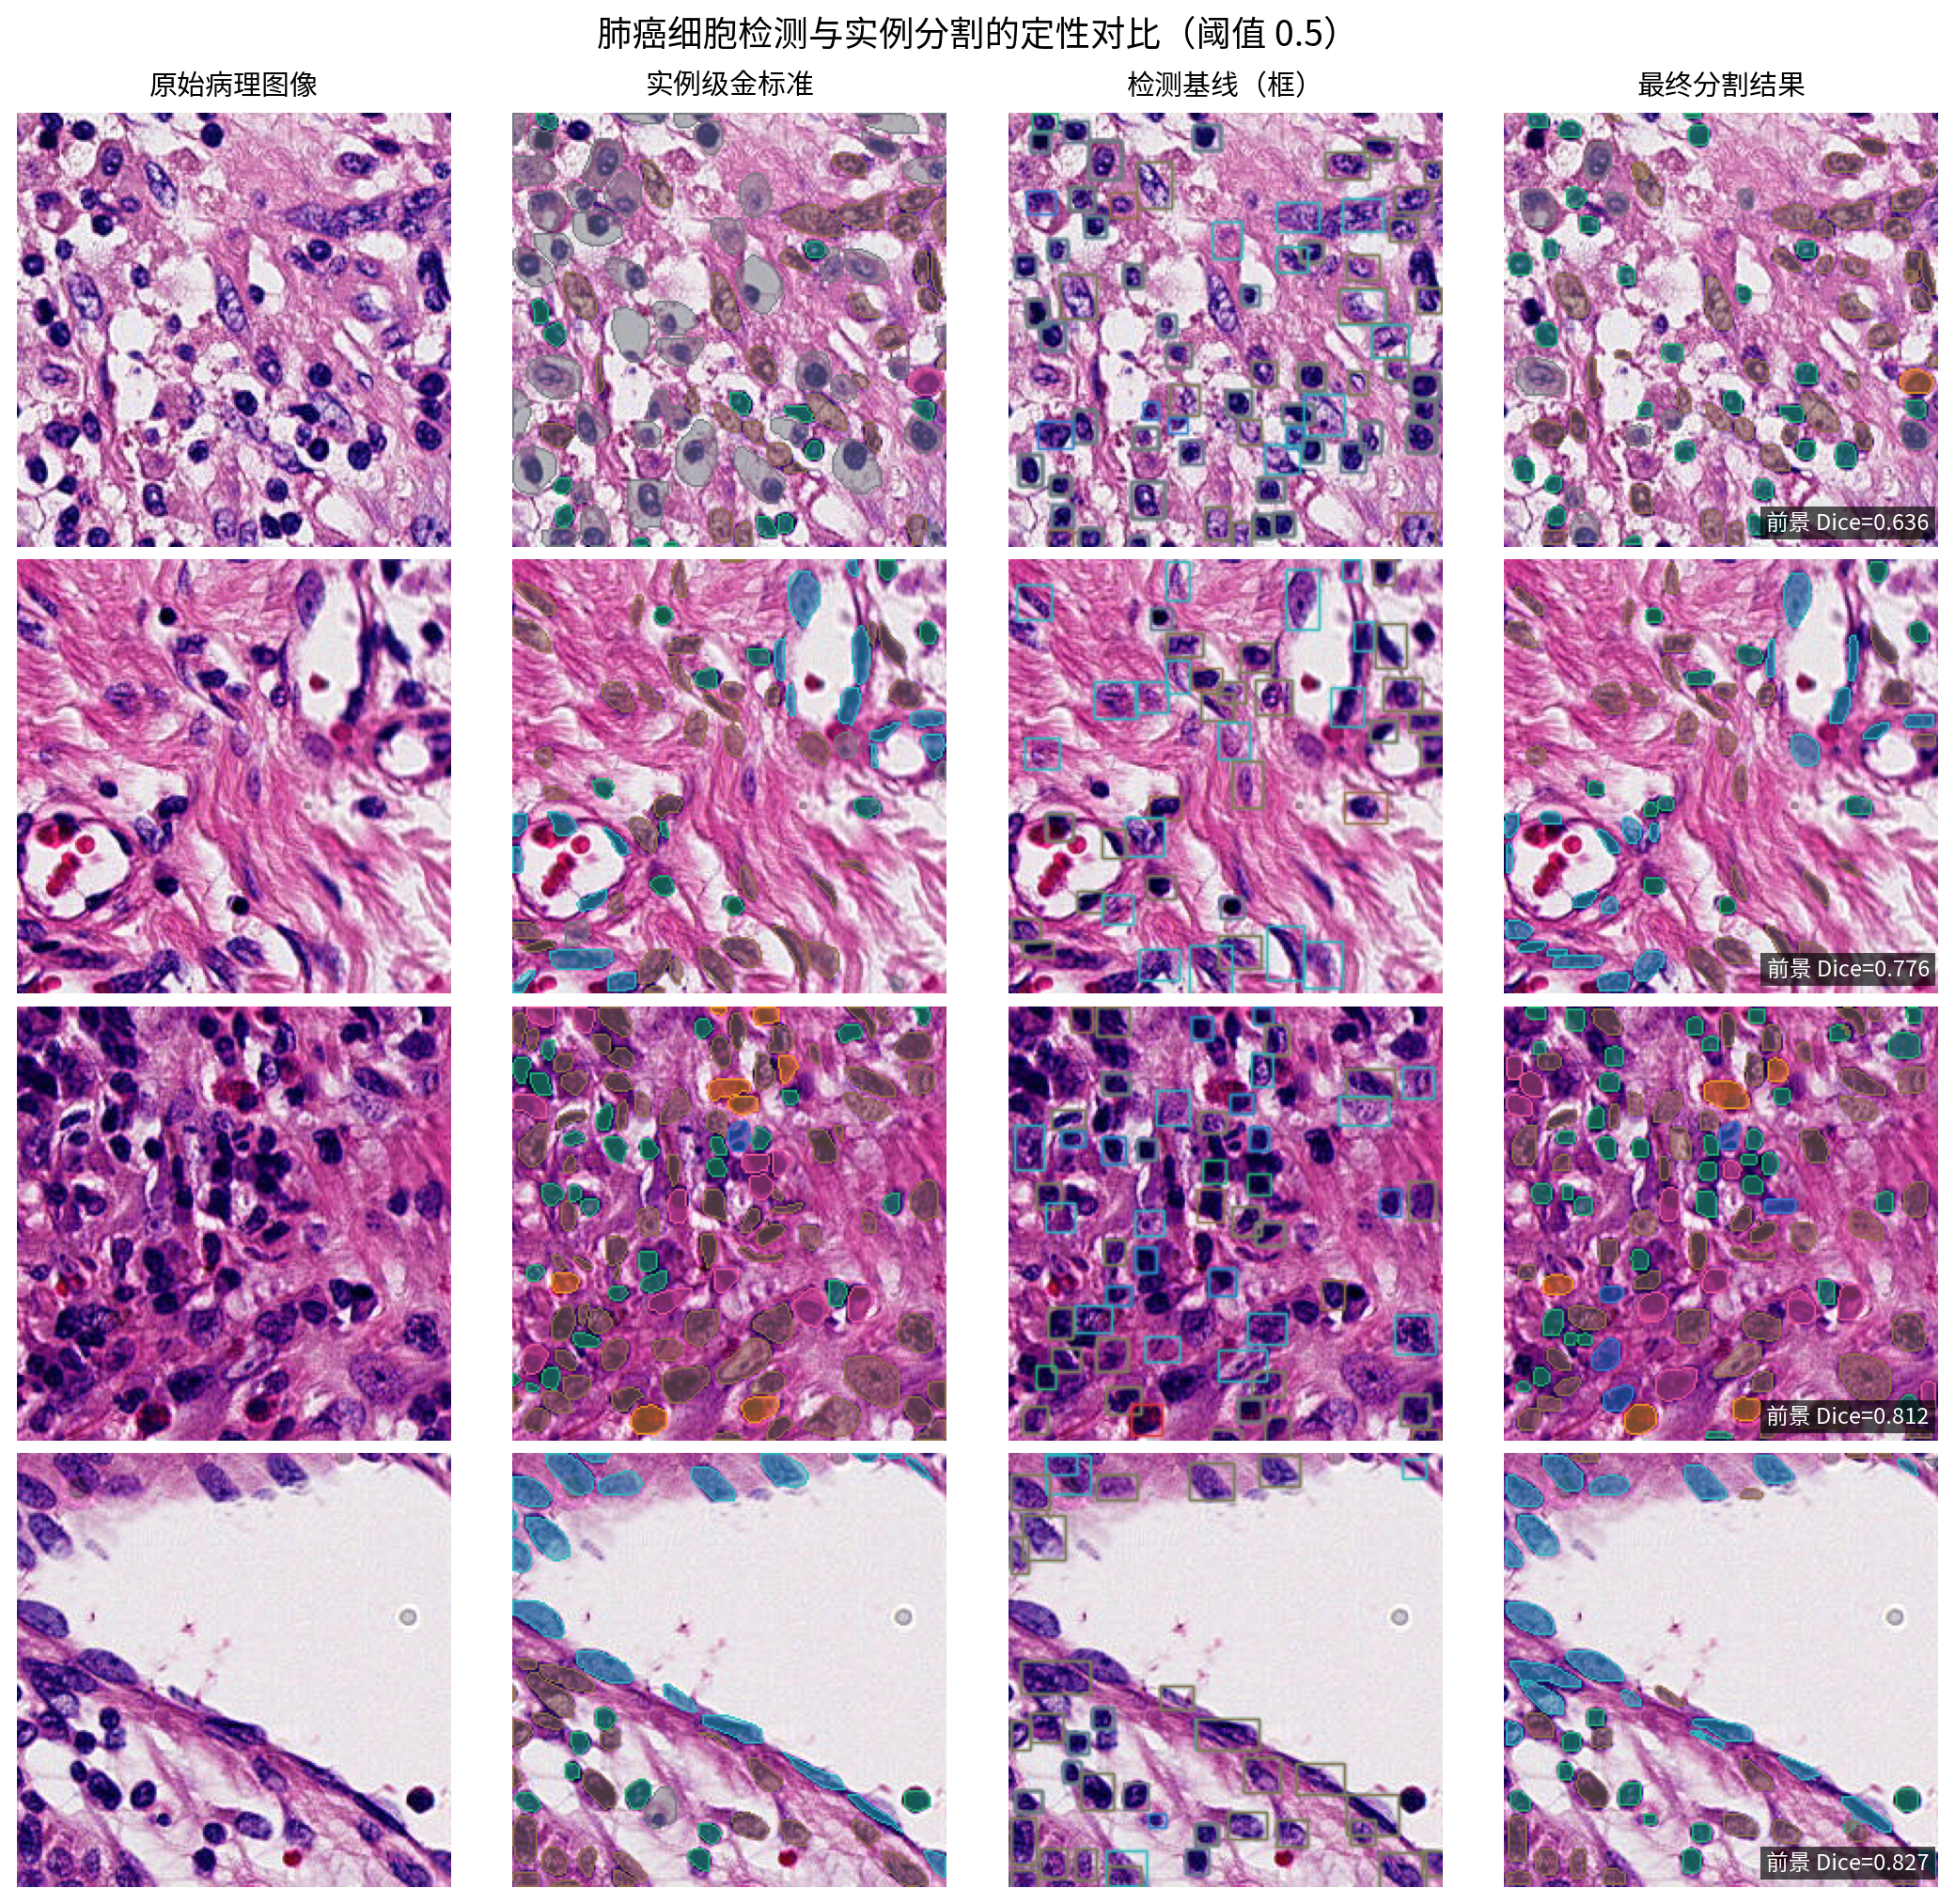
\includegraphics[width=0.92\textwidth]{chapters/lung_native_segmentation_final4000_4x4_20260901.png}
  \caption{肺癌细胞检测与实例分割的定性结果}
  \label{fig:lung_native_segmentation_final4000}
\end{figure}
图~\ref{fig:lung_native_segmentation_final4000} 按“原始病理图像--实例级金标准--历史检测基线--最终分割结果”四列展示代表性样本。样本依据前景 Dice 从低到高的分布位置选取，既包含较稳定案例，也保留一个相对困难案例。最终模型能够为肿瘤细胞、淋巴细胞、中性粒细胞和间质相关细胞等密集目标生成独立轮廓，较框级输出提供了更细的形态信息；但在细胞拥挤、边界模糊和切片边缘区域仍可见漏分、粘连或轮廓偏移。图中 Dice 为阈值 0.5 下的图块级前景 Dice，用于说明轮廓覆盖情况，不等同于按类别汇总的 COCO Segm AP。

上述结果仍需结合数据规模理解。当前评价集只有 8 个图块，虽然已核查训练集与评价集之间不存在同名文件或完全相同的图像哈希，但在缺少完整临床病例清单的情况下，尚不能据此宣称严格的患者级独立。后续应在具有明确患者标识的外部队列上扩大样本量，统一嗜酸性粒细胞相关标签，并报告患者分层的置信区间，才能更充分评价联合检测--分割模型的泛化能力。


\subsection{AI-RVT 与 VIS-RVT 的一致性}
在 SXCH 外部验证队列中，AI-RVT 与 VIS-RVT 的切片级组内相关系数（intraclass correlation coefficient, ICC）为 0.881（$p=1.08\times10^{-64}$），患者级 ICC 为 0.861（$p=6.03\times10^{-10}$）。在 NCC\_Cohort2 与 SZCH 组成的独立测试数据中，切片级 ICC 为 0.861（$p=6.96\times10^{-273}$），患者级 ICC 进一步达到 0.931（$p=1.05\times10^{-38}$）。患者级聚合降低了单张切片取材差异的影响，因而获得了更稳定的一致性。

采用 10\% RVT 阈值划分 MPR 和 non-MPR 时，AI-RVT 与 VIS-RVT 在 84 例患者中的一致率为 95.2\%（80/84）。四例不一致病例中，t1、t3 和 t4 均位于 10\% 阈值附近，主要反映边界病例的连续值差异；t2 的 VIS-RVT 为 22\%，AI-RVT 为 8.56\%，高倍图像显示活性肿瘤与间质广泛交织，人工视觉评估可能因复杂间质结构而高估活性肿瘤比例。该结果同时说明，连续 RVT 比单一阈值标签保留了更多病理信息。

\begin{figure}[tb]
  \centering
  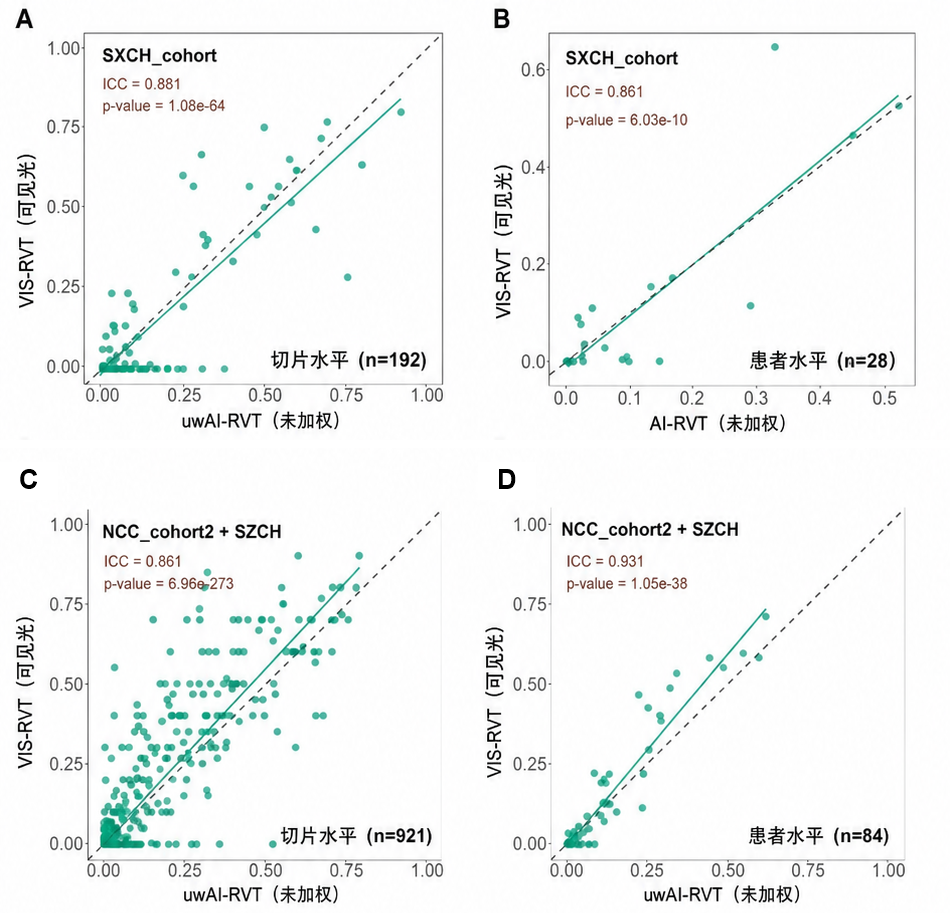
\includegraphics[width=0.70\textwidth]{chapters/lung_fig5_5_abef_precise_abcd_20260829.png}
  \caption{AI-RVT 与 VIS-RVT 的跨队列一致性}
  \label{fig:lung_concordance_quant}
\end{figure}
图~\ref{fig:lung_concordance_quant} 集中展示跨中心定量一致性。（A、B）分别为 SXCH 外部验证队列的切片级和患者级结果，ICC 为 0.881 和 0.861；（C、D）在 NCC\_Cohort2 与 SZCH 独立测试数据中重复评价，ICC 分别为 0.861 和 0.931。患者级聚合后仍保持较高一致性，说明模型并非只在个别切片上偶然吻合；相反，汇总同一患者多张 WSI 能够降低取材位置和局部异质性引起的波动。两组独立队列得到相近结论，也为 AI-RVT 的跨中心稳定性提供了证据。

\begin{figure}[tb]
  \centering
  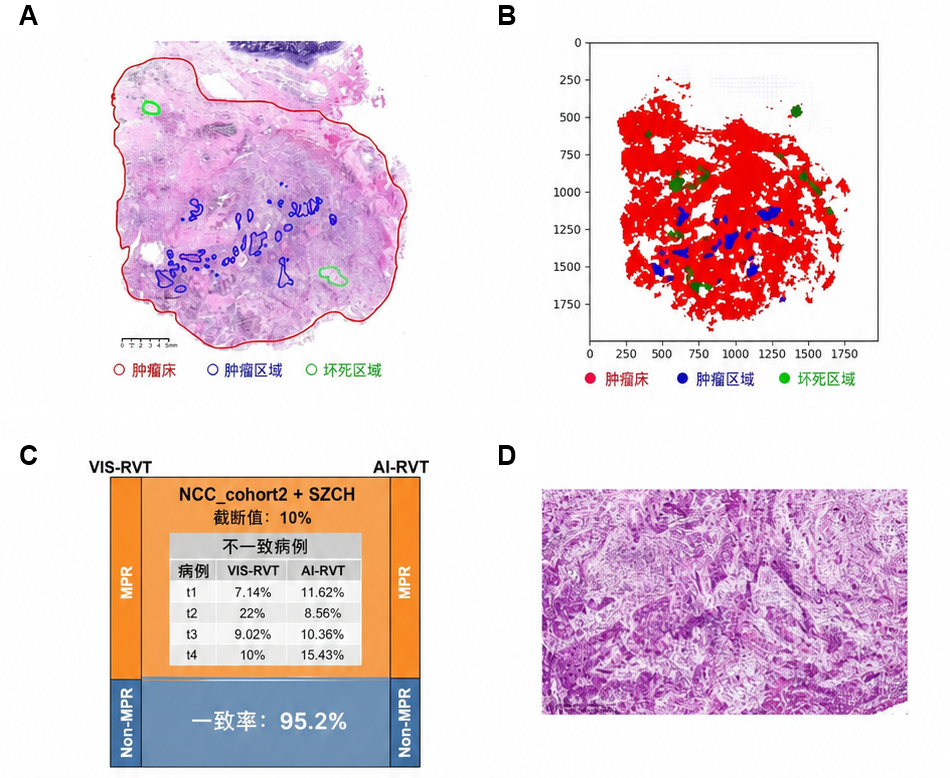
\includegraphics[width=0.72\textwidth]{chapters/lung_fig5_5_cdgh_precise_abcd_20260829.png}
  \caption{区域分割对照与 MPR 阈值判定}
  \label{fig:lung_concordance_cases}
\end{figure}
图~\ref{fig:lung_concordance_cases} 进一步解释一致性结果的病理来源。（A、B）将病理医师勾画的肿瘤床、活性肿瘤和坏死区域与 AI 分割结果并列，可见主体区域的空间判断总体一致，而差异主要位于复杂边界。（C）在 10\% RVT 阈值下比较 MPR 判定，84 例患者中有 80 例结论一致，一致率为 95.2\%。（D）展示差异较明显的病例：活性肿瘤与纤维化间质广泛交错，人工视觉估计容易受到局部高细胞密度区域影响。该病例说明，连续 AI-RVT 可保留阈值附近的细微差异，但不一致病例仍应结合原始 H\&E 形态复核。

\subsection{预后分析结果}
\subsubsection{阈值化 MPR 分层}
在 103 例总体预后队列中，VIS-RVT 和 AI-RVT 定义的 MPR 均能显著区分 DFS，log-rank 检验的 $p$ 值分别为 0.0011 和 0.00095。校正 ypN 后，VIS-RVT 定义的 non-MPR 风险比为 2.6（95\% CI：1.09--6.20，$p=0.031$），AI-RVT 定义的 non-MPR 风险比为 2.7（95\% CI：1.18--6.40，$p=0.019$）。两种方法对 OS 的分层均未达到显著水平，其中 VIS-RVT 的 $p=0.33$，AI-RVT 呈非显著趋势（$p=0.084$）。

在 78 例 non-pCR 亚组中，VIS-RVT 和 AI-RVT 定义的 MPR 仍能区分 DFS，$p$ 值分别为 0.023 和 0.021。多变量模型中，VIS-RVT 仅呈边界显著（HR=2.3，$p=0.061$），而 AI-RVT 定义的 non-MPR 仍与较短 DFS 独立相关（HR=2.5，95\% CI：1.04--6.0，$p=0.040$）。这一差异表明，自动化区域量化在残余肿瘤患者中可能比阈值化人工估计具有更稳定的风险识别能力。

\subsubsection{连续 RVT 分析}
将 RVT 作为连续变量可避免 10\% 阈值造成的信息损失。在总体队列中，连续 VIS-RVT 与 AI-RVT 的 DFS 风险比分别为 8.4（$p=0.009$）和 8.2（$p=0.022$）；在 non-pCR 亚组中，两者的风险比分别为 7.2（$p=0.018$）和 7.0（$p=0.037$）。二者效应方向和量级高度一致，但均未对 OS 显示稳定关联。这表明 RVT 更直接反映复发风险，而 OS 可能同时受到后续治疗、非肿瘤死亡和治疗后免疫生态等因素影响。

\begin{figure}[tb]
  \centering
  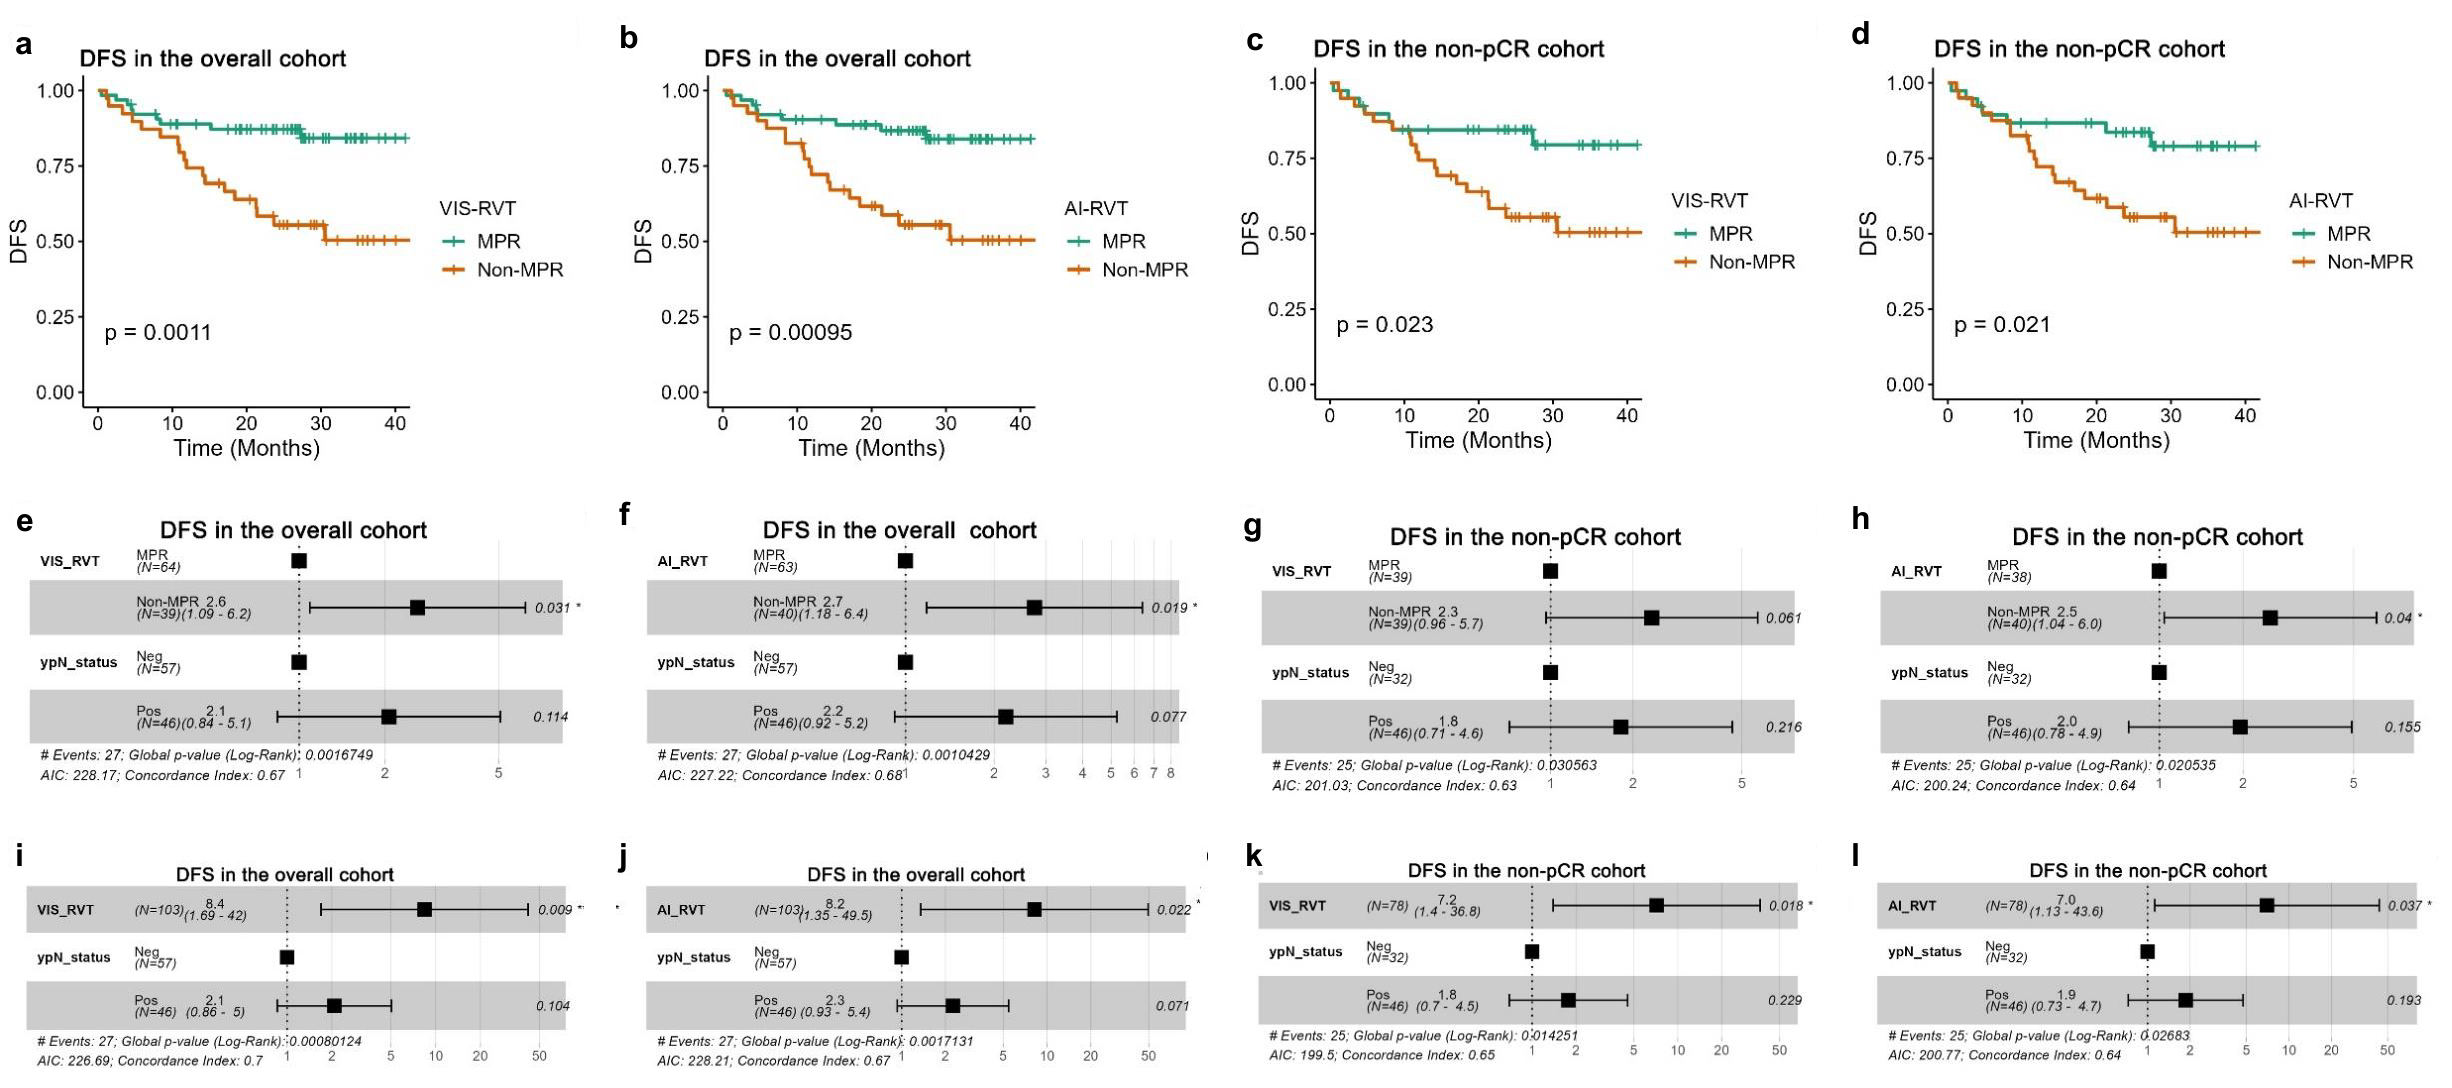
\includegraphics[width=\textwidth]{chapters/lung_rvt_survival_3x4_20260831.png}
  \caption{RVT 与无病生存期的关联}
  \label{fig:lung_rvt_survival}
\end{figure}
图~\ref{fig:lung_rvt_survival} 从阈值分层和连续变量两个角度说明 RVT 与无病生存期的关系。第一行（a--d）给出 Kaplan--Meier 曲线：（a、b）分别采用 VIS-RVT 与 AI-RVT，在总体队列中划分 MPR 和 non-MPR；（c、d）则将同样的分析限制在 non-pCR 患者中，以排除完全缓解病例对结果的主导作用。四幅曲线均显示 non-MPR 患者的 DFS 较差，说明两种 RVT 评估均可形成与临床结局相关的患者分层。

第二行（e--h）对应多变量 Cox 分析，其中（e、f）为总体队列，（g、h）为 non-pCR 亚组。在校正 ypN 等临床因素后，总体队列中两种 RVT 定义仍保留独立的 DFS 风险信息，AI-RVT 定义的 non-MPR 风险比为 2.7。在 non-pCR 亚组中，VIS-RVT 的关联减弱，而 AI-RVT 的关联仍达到统计学显著。该结果支持自动量化评估具有一定的预后分层价值，但不能仅依据生存关联直接推断其测量重复性。

第三行（i--l）不再使用 10\% 二分阈值，而是直接把 RVT 作为连续变量进入模型；（i、j）分析总体队列，（k、l）分析 non-pCR 亚组。两种评估在不同人群中的效应方向保持一致。连续分析保留了治疗反应程度的梯度信息，避免将 9\% 与 11\% 这类数值接近的病例仅按阈值分到不同组，可作为 MPR 分层分析的补充。

\subsection{空间免疫分析结果}
\subsubsection{距离依赖的单一细胞效应}
在具有残余肿瘤的 NCC 和 SZCH 患者中，$50$--$700\,\mu\mathrm{m}$ 各距离范围的细胞组成总体一致：成纤维细胞最丰富，其次为淋巴细胞；浆细胞、组织细胞、中性粒细胞和内皮细胞处于中等水平；嗜酸性粒细胞因数量过少而不纳入预后分析。

既往研究已表明，肿瘤免疫微环境不仅取决于细胞丰度，还取决于免疫细胞的空间组织、细胞邻域和浸润形态\cite{keren2018structured,saltz2018spatial}；在早期非小细胞肺癌中，TIL 的空间结构亦与复发风险相关\cite{corredor2019spatil}。空间 Cox 分析显示，不同细胞的预后作用具有明确的距离依赖性。对于 DFS，肿瘤边界 $50\,\mu\mathrm{m}$ 内高中性粒细胞密度与较差 DFS 相关（log-rank $p=0.040$），同一区域高内皮细胞密度也与较差 DFS 相关（$p=0.014$）。同时纳入 ypN 和 AI-RVT 后，内皮细胞密度仍是独立复发风险因素（HR=2.9，95\% CI：1.07--7.8，$p=0.036$），而中性粒细胞对 DFS 不再独立显著。

OS 呈现另一组互补信号。$50\,\mu\mathrm{m}$ 内高中性粒细胞密度与较差 OS 相关（log-rank $p=0.0089$），$700\,\mu\mathrm{m}$ 范围内高淋巴细胞密度则与更好 OS 相关（$p=0.032$）。在校正 ypN 和 AI-RVT 的 Firth Cox 模型中，远端淋巴细胞仍是保护因素（HR=0.15，95\% CI：0.015--0.79，$p=0.024$），近端中性粒细胞则是风险因素（HR=7.5，95\% CI：1.5--76，$p=0.012$）。这说明紧邻肿瘤的中性粒细胞富集和更广空间内的淋巴细胞浸润分别刻画局部不利炎症生态与整体抗肿瘤免疫能力。

\begin{table}[htbp]
  \centering
  \caption{空间免疫特征的预后效应}
  \label{tab:lung_spatial_effects}
  \resizebox{0.98\textwidth}{!}{%
  \begin{tabular}{lllll}
    \toprule
    终点 & 空间特征 & 单因素 $p$ 值 & 多变量 HR（95\% CI） & 多变量 $p$ 值 \\
    \midrule
    DFS & 中性粒细胞，$50\,\mu\mathrm{m}$ & 0.040 & 1.2（0.47--3.3） & 0.663 \\
    DFS & 内皮细胞，$50\,\mu\mathrm{m}$ & 0.014 & 2.9（1.07--7.8） & 0.036 \\
    OS & 中性粒细胞，$50\,\mu\mathrm{m}$ & 0.0089 & 7.5（1.5--76） & 0.012 \\
    OS & 淋巴细胞，$700\,\mu\mathrm{m}$ & 0.032 & 0.15（0.015--0.79） & 0.024 \\
    \bottomrule
  \end{tabular}}
\end{table}

\begin{figure}[tb]
  \centering
  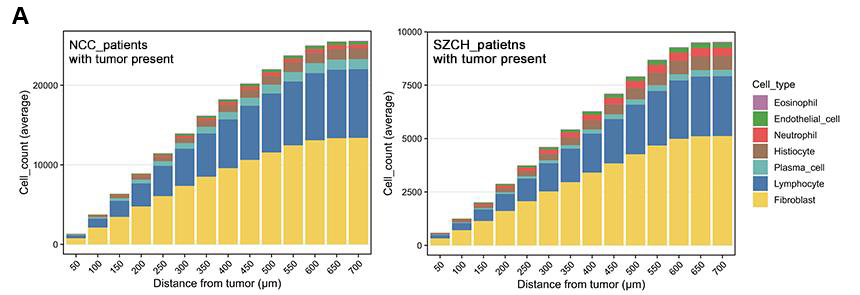
\includegraphics[width=0.82\textwidth]{chapters/lung_fig5_7_a_precise_A_20260829.png}
  \caption{跨中心不同径向范围的细胞组成}
  \label{fig:lung_spatial_composition}
\end{figure}
图~\ref{fig:lung_spatial_composition} 首先比较 NCC 与 SZCH 残余肿瘤患者在 $50$--$700\,\mu\mathrm{m}$ 径向范围内的累积细胞组成。两队列随距离增加呈现相近的总体趋势，成纤维细胞和淋巴细胞占比较高，中性粒细胞、内皮细胞等类别所占比例较低但具有特定空间分布。跨中心组成的一致性说明，后续预后关联并非由某一个中心特有的细胞构成所驱动；同时，累计数量随距离增加并不意味着风险效应同步增强，真正具有解释价值的是细胞类别、肿瘤距离和临床终点三者的联合关系。

\begin{figure}[tb]
  \centering
  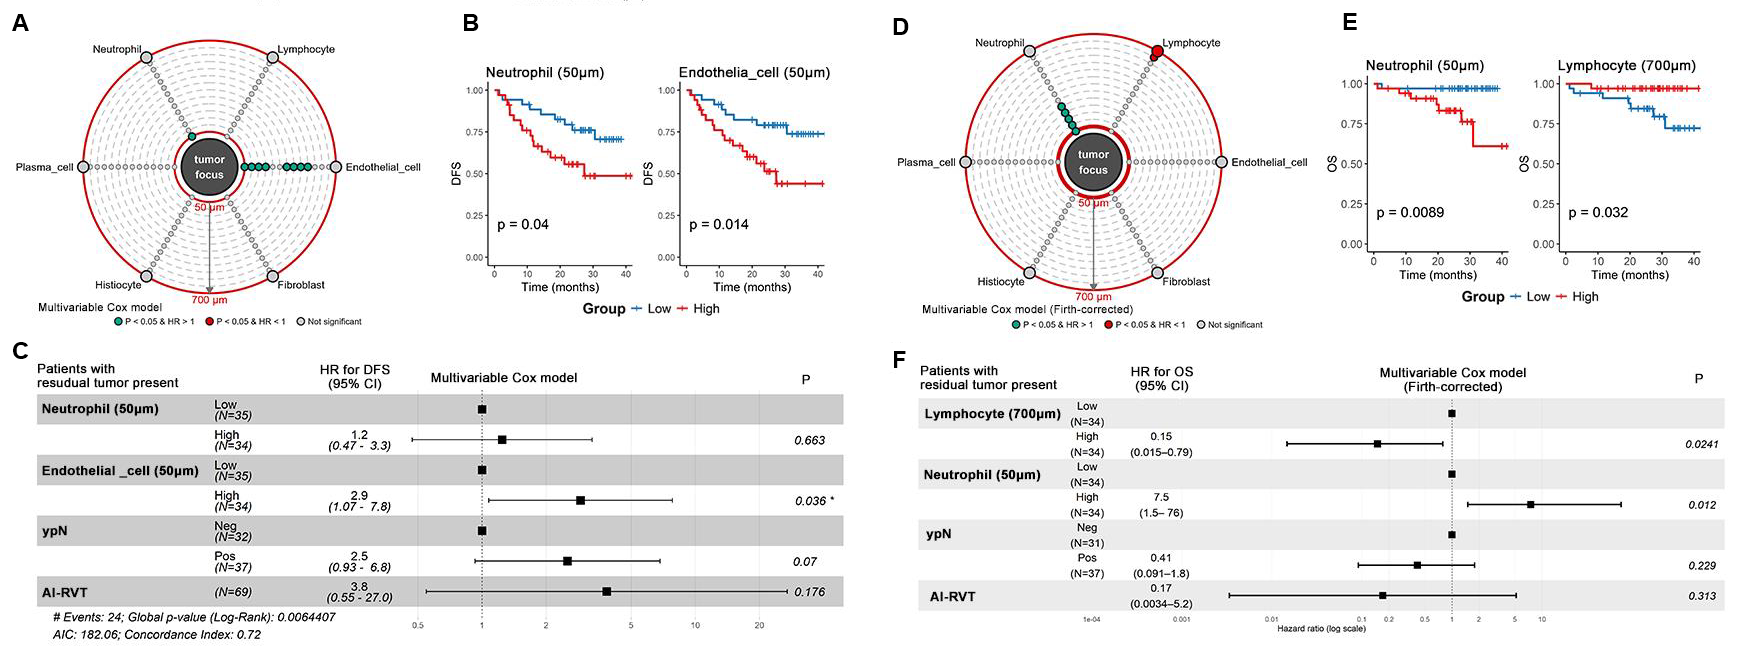
\includegraphics[width=\textwidth]{chapters/lung_spatial_survival_horizontal_20260831.png}
  \caption{空间免疫特征与生存结局}
  \label{fig:lung_spatial_survival}
\end{figure}
图~\ref{fig:lung_spatial_survival} 将距离扫描结果与生存分析对应起来。左侧（A--C）聚焦 DFS：径向扫描提示肿瘤边界近端的中性粒细胞和内皮细胞与较差结局相关，Kaplan--Meier 曲线展示高低密度组差异，多变量模型进一步校正 ypN 与 AI-RVT。校正后，$50\,\mu\mathrm{m}$ 内内皮细胞仍保持独立风险作用（HR=2.9，$p=0.036$），而中性粒细胞的 DFS 效应减弱。右侧（D--F）采用同样结构分析 OS，并针对较少事件使用 Firth 校正。$50\,\mu\mathrm{m}$ 内高中性粒细胞密度是风险因素（HR=7.5，$p=0.012$），$700\,\mu\mathrm{m}$ 内高淋巴细胞密度则表现为保护因素（HR=0.15，$p=0.024$）。结果说明，紧邻肿瘤的局部促肿瘤炎症与更大范围的抗肿瘤免疫浸润是方向相反但可同时存在的空间生态。

\subsubsection{淋巴细胞--中性粒细胞联合表型}
根据 $700\,\mu\mathrm{m}$ 内淋巴细胞密度和 $50\,\mu\mathrm{m}$ 内中性粒细胞密度，将残余肿瘤患者划分为四种 Lym+Neu 空间免疫表型。联合表型能够区分 DFS（log-rank $p=0.026$）：低淋巴细胞/高中性粒细胞组的 DFS 最差，高淋巴细胞/低中性粒细胞组最好；但该 DFS 关联在多变量模型中未保持独立显著。

相比之下，联合表型对 OS 的区分更强（log-rank $p=0.0092$）。在校正 ypN 和 AI-RVT 的 Firth Cox 模型中，低淋巴细胞/高中性粒细胞表型相对于高淋巴细胞/低中性粒细胞表型仍与不良 OS 独立相关，HR 为 31（95\% CI：3.2--402，$p=0.0011$）。较宽的置信区间反映 OS 事件数有限，但效应方向与单一细胞分析完全一致：近端中性粒细胞富集与远端淋巴细胞缺失共同构成最不利的治疗后免疫结构。

\begin{figure}[tb]
  \centering
  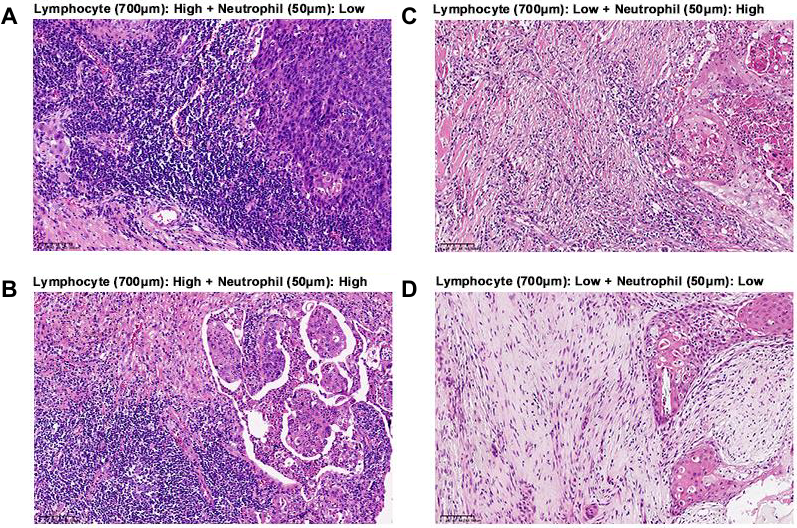
\includegraphics[width=0.92\textwidth]{chapters/lung_combined_morphology_rotated_20260831.png}
  \caption{淋巴细胞--中性粒细胞联合表型的病理形态}
  \label{fig:lung_combined_morphology}
\end{figure}
图~\ref{fig:lung_combined_morphology} 展示四种联合表型的代表性 H\&E 区域。左列依次为（A）高淋巴细胞/低中性粒细胞和（B）高淋巴细胞/高中性粒细胞，右列依次为（C）低淋巴细胞/高中性粒细胞和（D）低淋巴细胞/低中性粒细胞。这里的“高/低”分别依据 $700\,\mu\mathrm{m}$ 范围内的淋巴细胞密度与 $50\,\mu\mathrm{m}$ 范围内的中性粒细胞密度定义，并非仅凭所展示的局部视野判断。该划分同时编码较大范围的适应性免疫浸润和紧邻肿瘤的炎症反应，比单独统计某一类细胞更接近真实肿瘤微环境。

\begin{figure}[tb]
  \centering
  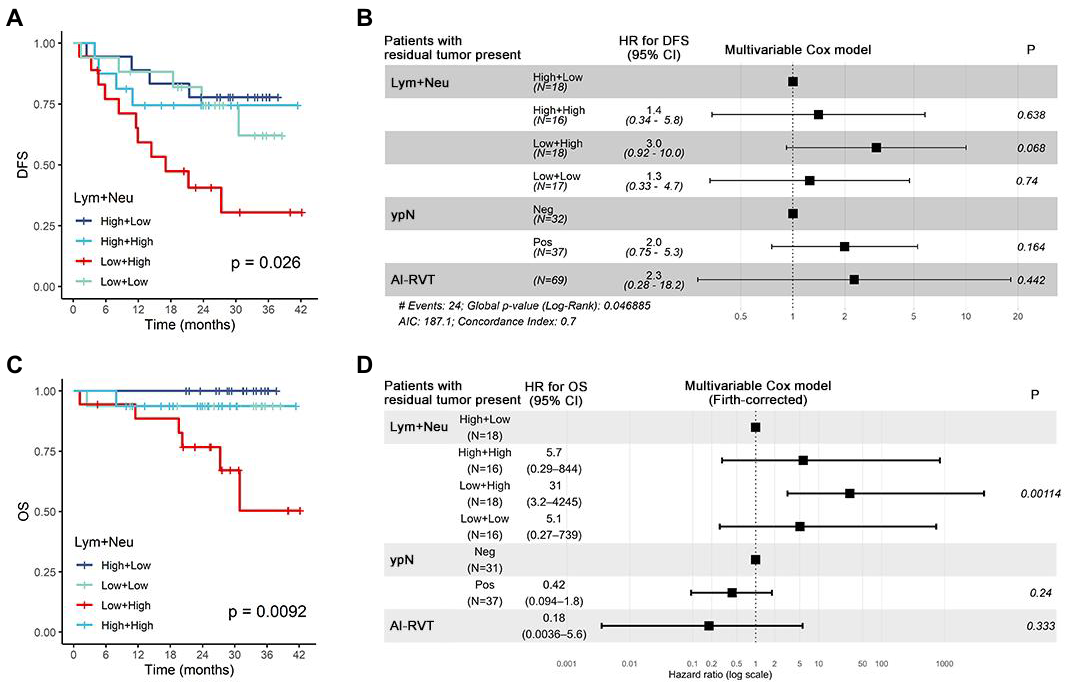
\includegraphics[width=0.95\textwidth]{chapters/lung_combined_survival_abcd_20260831.png}
  \caption{淋巴细胞--中性粒细胞联合表型与生存结局}
  \label{fig:lung_combined}
\end{figure}
图~\ref{fig:lung_combined} 分析上述四种联合表型与生存结局的关系。（A、B）显示联合表型能够区分 DFS，其中低淋巴/高中性组曲线最差、高淋巴/低中性组最好；校正临床变量后，DFS 关联减弱，说明复发风险仍较多受到残余肿瘤负荷和淋巴结状态影响。（C、D）显示联合表型对 OS 的分层更明显。在 Firth 校正模型中，低淋巴/高中性组相对于高淋巴/低中性组仍具有显著较高风险，方向与图~\ref{fig:lung_spatial_survival} 的单细胞结果一致。由于 OS 事件数有限、置信区间较宽，该结果更适合作为具有生物学一致性的风险信号，仍需在更大规模前瞻性队列中验证。

\subsection{细胞实例特征分布分析}
为检验渐进式视觉语言预训练是否改善肺鳞癌病理细胞的实例表征，本文对同一批标注实例分别提取未经额外医学预训练的 GLIP-ZS 特征与渐进式预训练后的特征，并采用一致的 PCA 与 t-SNE 参数进行降维。参与比较的类别包括肿瘤细胞、淋巴细胞、中性粒细胞、浆细胞、血管内皮细胞和纤维间质细胞等。

\begin{figure}[tb]
  \centering  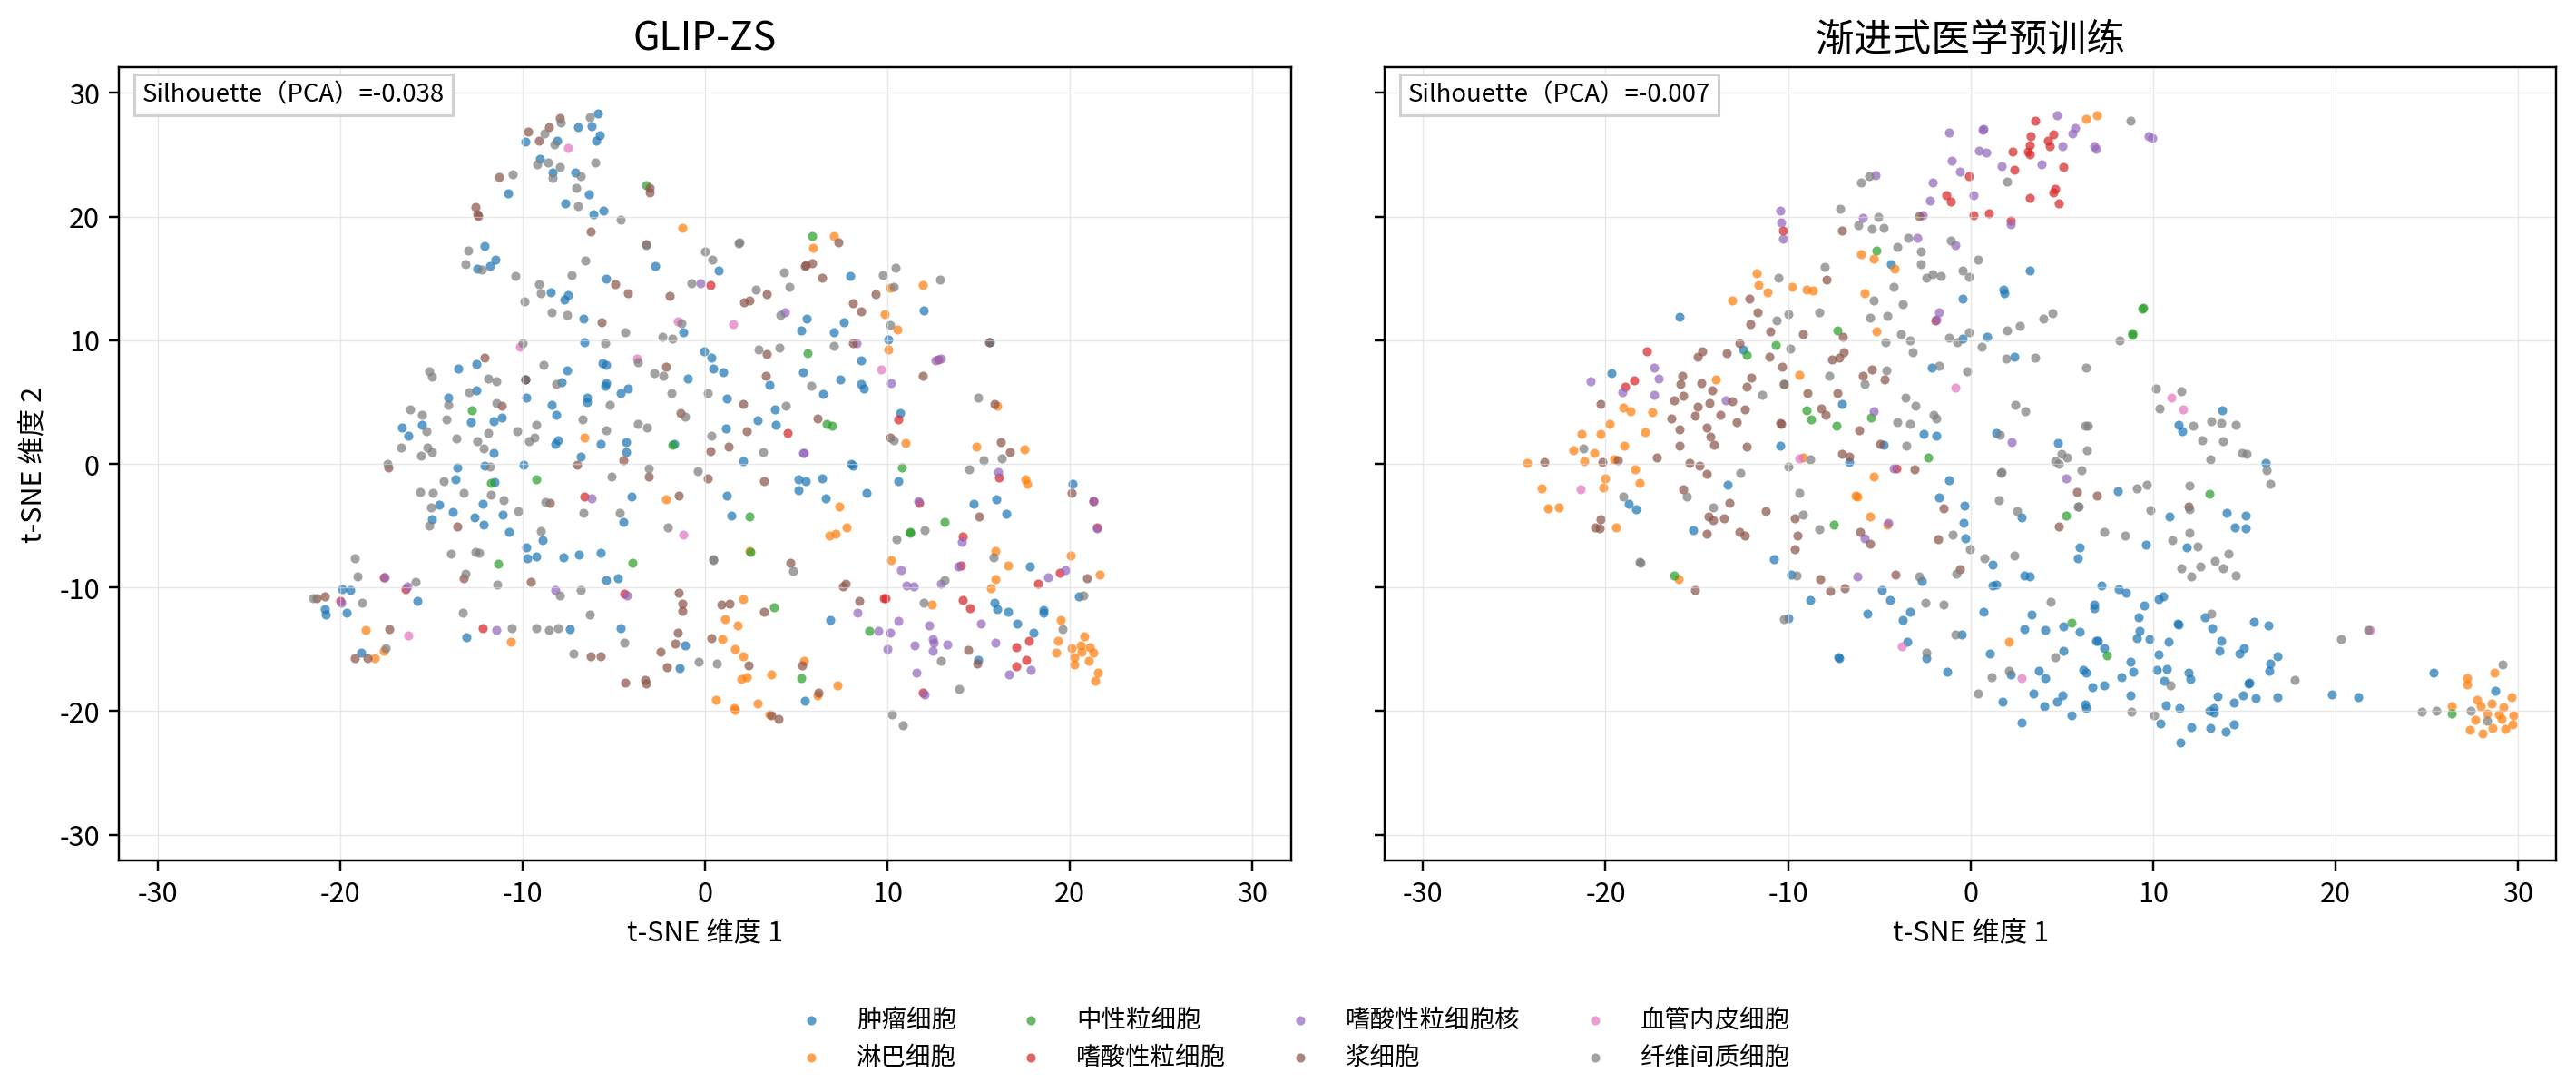
\includegraphics[width=0.84\textwidth]{figures/figure5_lungscc_tsne_centered_20260823.png}  \caption{GLIP-ZS 与渐进式预训练模型的肺鳞癌细胞实例特征分布}  \label{fig:lung_progressive_tsne}
\end{figure}
图~\ref{fig:lung_progressive_tsne} 显示，渐进式预训练后同类样本的局部聚集趋势更加明显，PCA 特征上的轮廓系数由 $-0.038$ 提高至 $-0.007$，t-SNE 平面上的轮廓系数由 $-0.149$ 提高至 $-0.056$。指标仍为负值，说明不同细胞形态之间依然存在较强重叠，因此该结果应理解为可分性的相对改善，而不是类别已经完全分离。左右子图仅通过二维平移进行显示居中，样本间距离和评价指标均未改变。

\section{本章小结}
本研究将治疗后 LUSC 的病理分析拆分为三个相互衔接且可解释的层次。第一层通过多尺度区域分类量化 RVT，解决人工估计工作量大和重复性不足的问题；第二层利用视觉语言基础模型统一异构细胞标签空间，在有限域内标注下识别七类肿瘤周围非肿瘤细胞；第三层将细胞位置转换为相对肿瘤边界的空间密度，以解释具有相似 RVT 患者之间仍然存在的预后差异。

AI-RVT 在外部验证和独立测试数据中均与 VIS-RVT 高度一致，患者级 ICC 达到 0.861--0.931，10\% 阈值下的一致率为 95.2\%。更重要的是，AI-RVT 的价值不仅是复现病理医师的读数。在 non-pCR 人群中，AI-RVT 定义的 non-MPR 在校正 ypN 后仍能独立预测 DFS，而 VIS-RVT 仅达到边界显著。连续 RVT 的风险效应又明显强于简单的 MPR 二分，说明治疗反应本质上是连续谱，强制阈值化会损失临床相关信息。

RVT 对 DFS 的稳定作用和空间免疫特征对 OS 的补充作用具有生物学合理性。RVT 更直接反映新辅助治疗后的局部肿瘤清除程度，因此首先关联复发；OS 则受到宿主免疫状态、后续治疗及全身疾病过程的共同影响。近端中性粒细胞富集可能对应免疫抑制、组织损伤和促肿瘤炎症，远端淋巴细胞丰富则更可能反映广泛而持续的抗肿瘤免疫。将两者组合后，低淋巴细胞/高中性粒细胞表型在校正 AI-RVT 与 ypN 后仍显示最高 OS 风险，说明空间免疫表型能够提供超越残余肿瘤负荷的互补信息。

本研究仍存在若干限制。首先，研究为回顾性设计，OS 事件数较少，尽管采用 Firth 校正降低了估计偏倚，HR=31 的置信区间仍较宽，需要更大规模前瞻性多中心队列验证。其次，每张 WSI 以最大肿瘤灶代表周边微环境，尚未完全覆盖多灶和区域异质性。再次，细胞类别依据 H\&E 形态预测，不能替代免疫组化或空间组学对功能亚型的鉴定。最后，当前方法主要计算到肿瘤边界的径向距离，后续可进一步引入细胞邻接图、聚集结构和三级淋巴结构等高阶空间特征。

本章的创新主要体现在以下三个方面。

第一，提出模拟病理医师“器官--组织--细胞”阅片过程的多尺度 WSI 模型，通过空间对齐的感受野扩展和面积加权融合生成连续 AI-RVT，在外部与独立数据中实现稳定的患者级一致性。

第二，提出面向异构病理细胞数据的渐进式视觉语言预训练策略，将公共多类核数据、目标域肿瘤/间质粗标注及少量八类精细标注依次用于域适配，在相同流程下显著优于 Mask R-CNN 和未经额外预训练的 GLIP。

第三，建立以肿瘤边界为参照的 $50$--$700\,\mu\mathrm{m}$ 空间免疫量化方法，发现近端中性粒细胞和远端淋巴细胞具有方向相反的 OS 效应，并构建能够在校正 AI-RVT 与 ypN 后继续分层 OS 的 Lym+Neu 联合表型。

本章围绕肺鳞癌新辅助免疫化疗后的疗效与预后评估，形成了“多尺度区域识别--连续 AI-RVT--多类细胞检测--空间密度建模--联合生存分析”的完整技术链。终稿结果表明，AI-RVT 能够高一致性复现人工 RVT，并对总体及 non-pCR 人群的 DFS 提供稳定信息；空间免疫分析进一步揭示 $50\,\mu\mathrm{m}$ 近端中性粒细胞的风险作用和 $700\,\mu\mathrm{m}$ 远端淋巴细胞的保护作用。二者构成的低淋巴细胞/高中性粒细胞表型识别出残余肿瘤患者中 OS 最差的亚群，从而把自动病理反应评估扩展为可解释的术后风险分层框架。
